\section{Further Evaluation Details}
\label{sec:newResults}

In this appendix we provide further details on how we find suitable parameter values for the initial and periodic proximity verification, and describe additional experimental results such as the effect of system load on proximity verification execution.


\subsection{Initial Proximity Verification}
\label{sec:newResults:distanceBound}

In Section~\ref{sec:evaluation:parameters}, we outlined a three-step approach to determine suitable parameter values for proximity verification. Here, we provide further details on each of these steps. 


\begin{figure}[t]
  \centering
    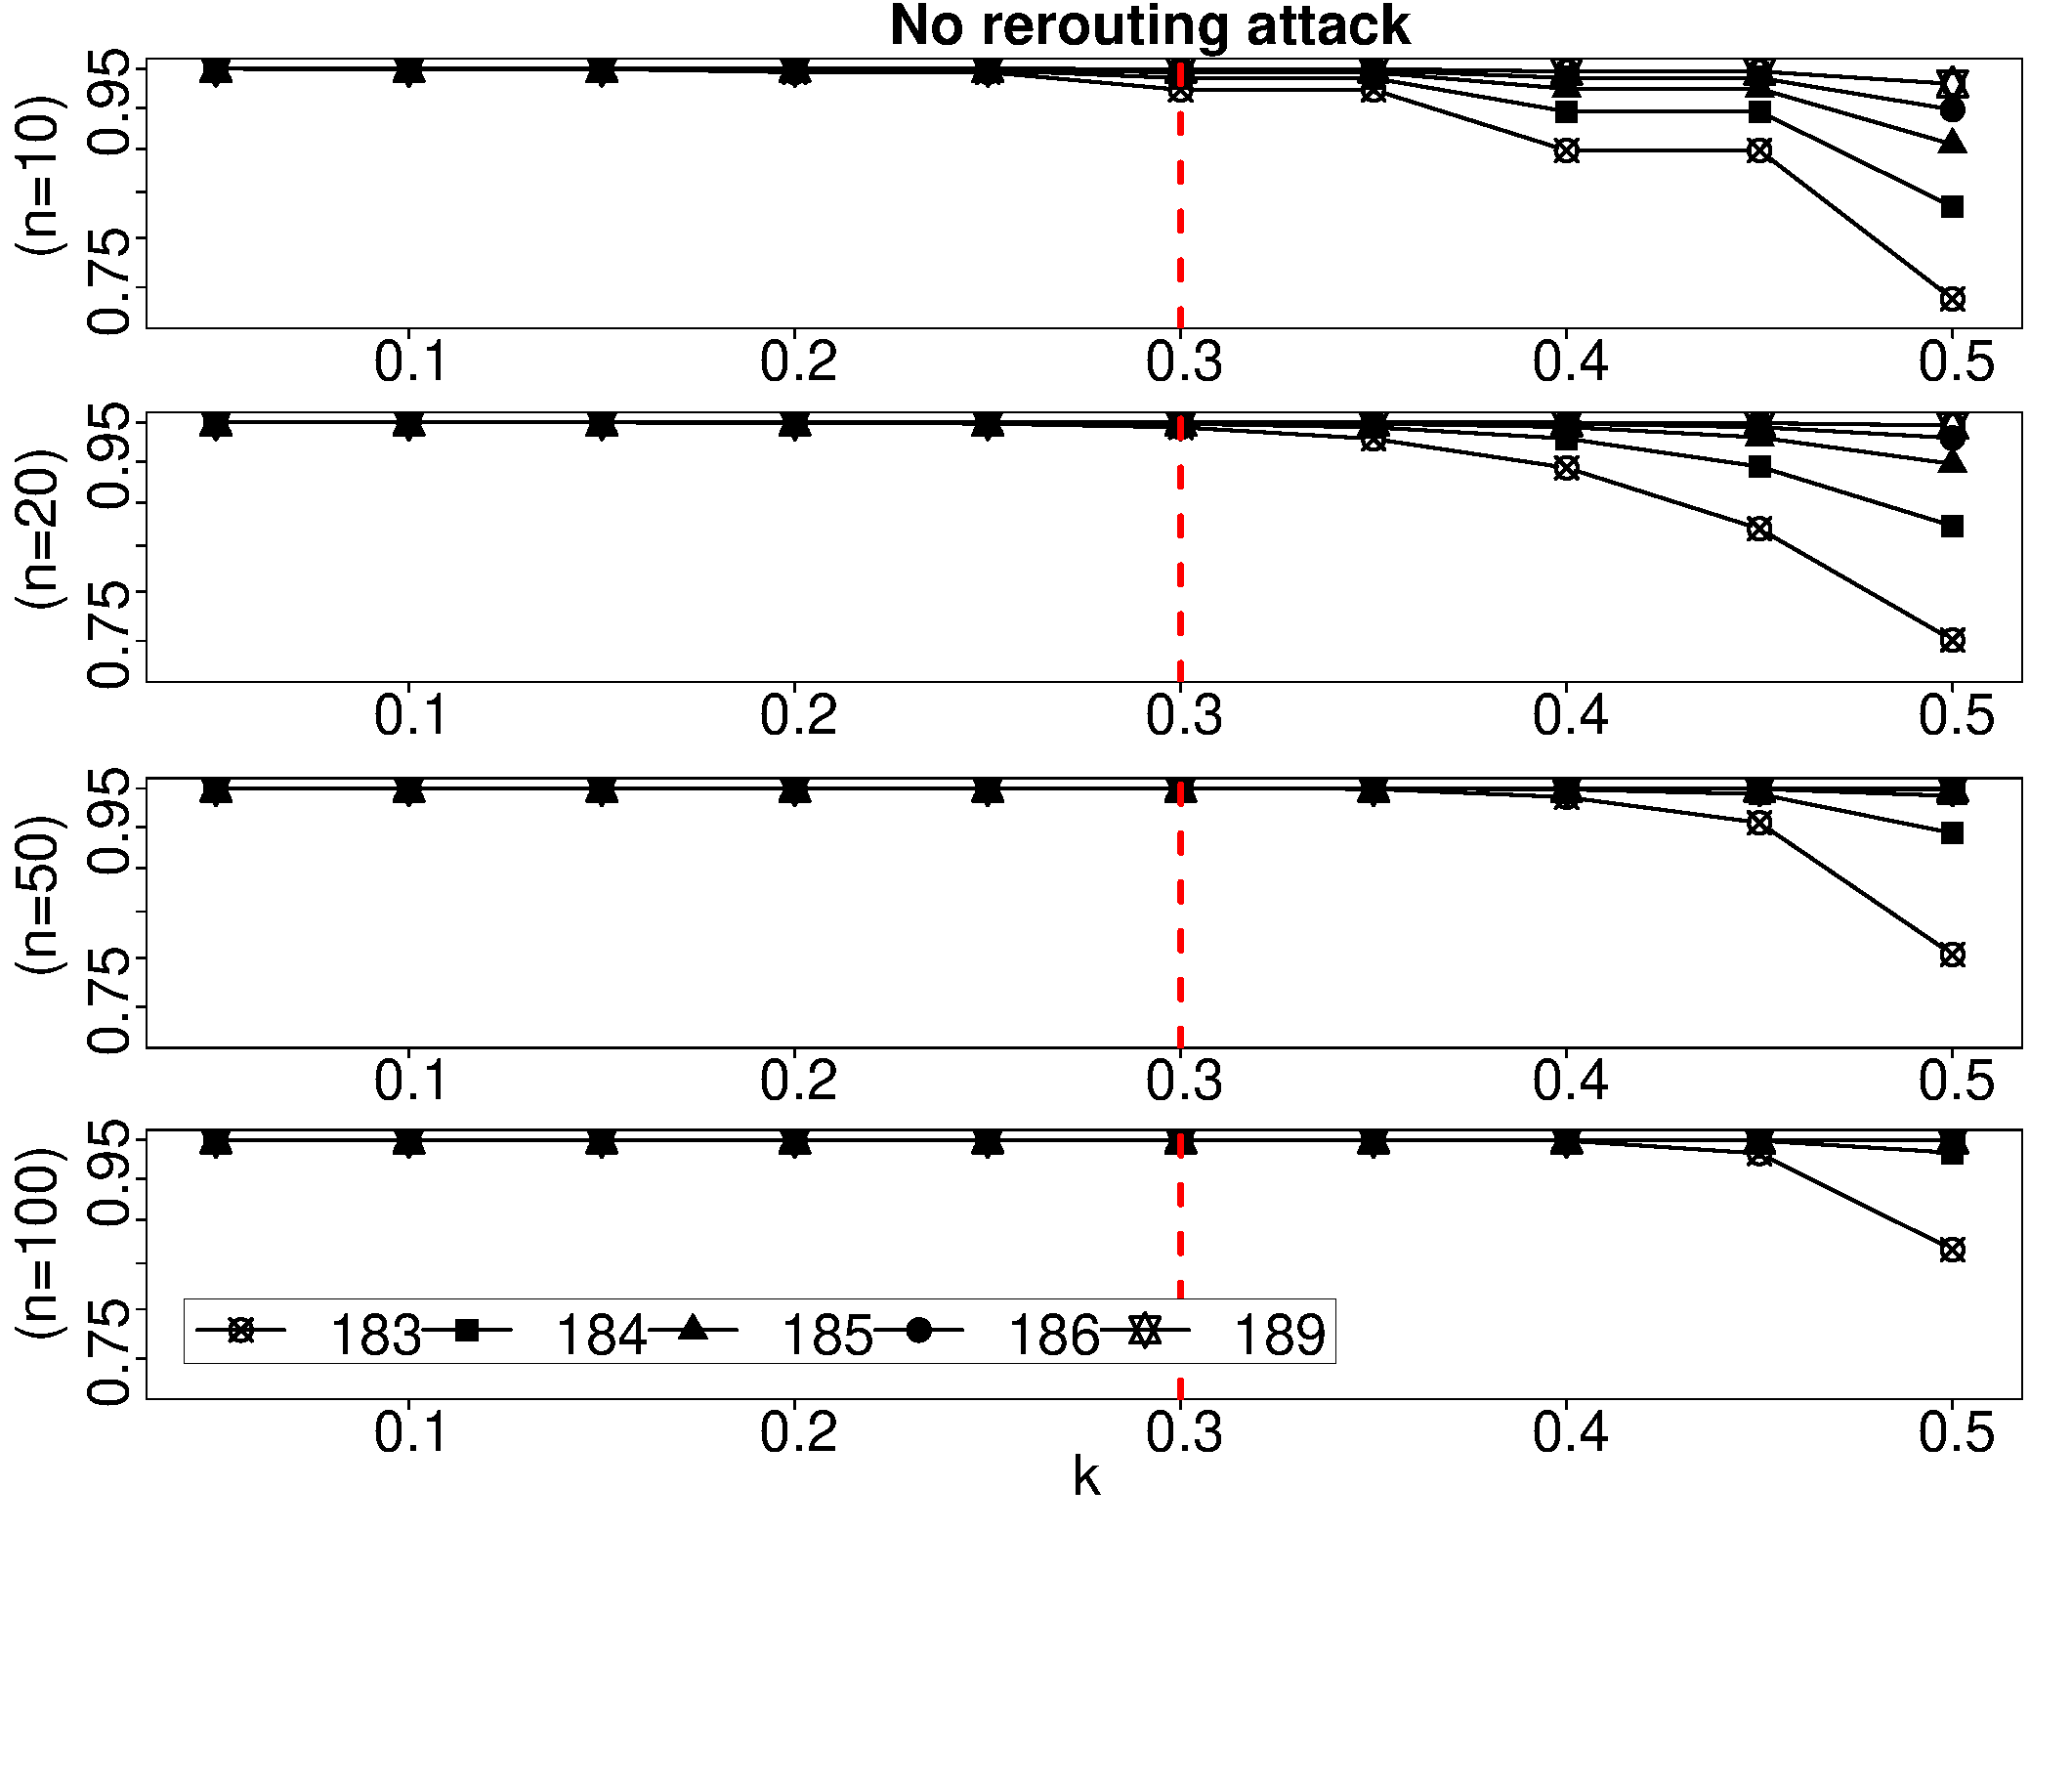
\includegraphics[trim={0 5cm 0 0}, clip, width=\linewidth]{data/fx3_data/timeRound.pdf}
    \caption{Legitimate attestation success probability for different \connect values. The chosen value \connect $=186\ \mu s$ gives success probability $0.999999977$ for number of trials at least 15 out of $n=50$ rounds when $k=0.3$.}
	\figsaver
    \label{graph:diffTh}
\end{figure}


\begin{figure}[t]
  \centering
    %\includegraphics[trim={0 0 0 0}, clip, width=0.4\linewidth]{data/graph/CDF_Latency.pdf}
    %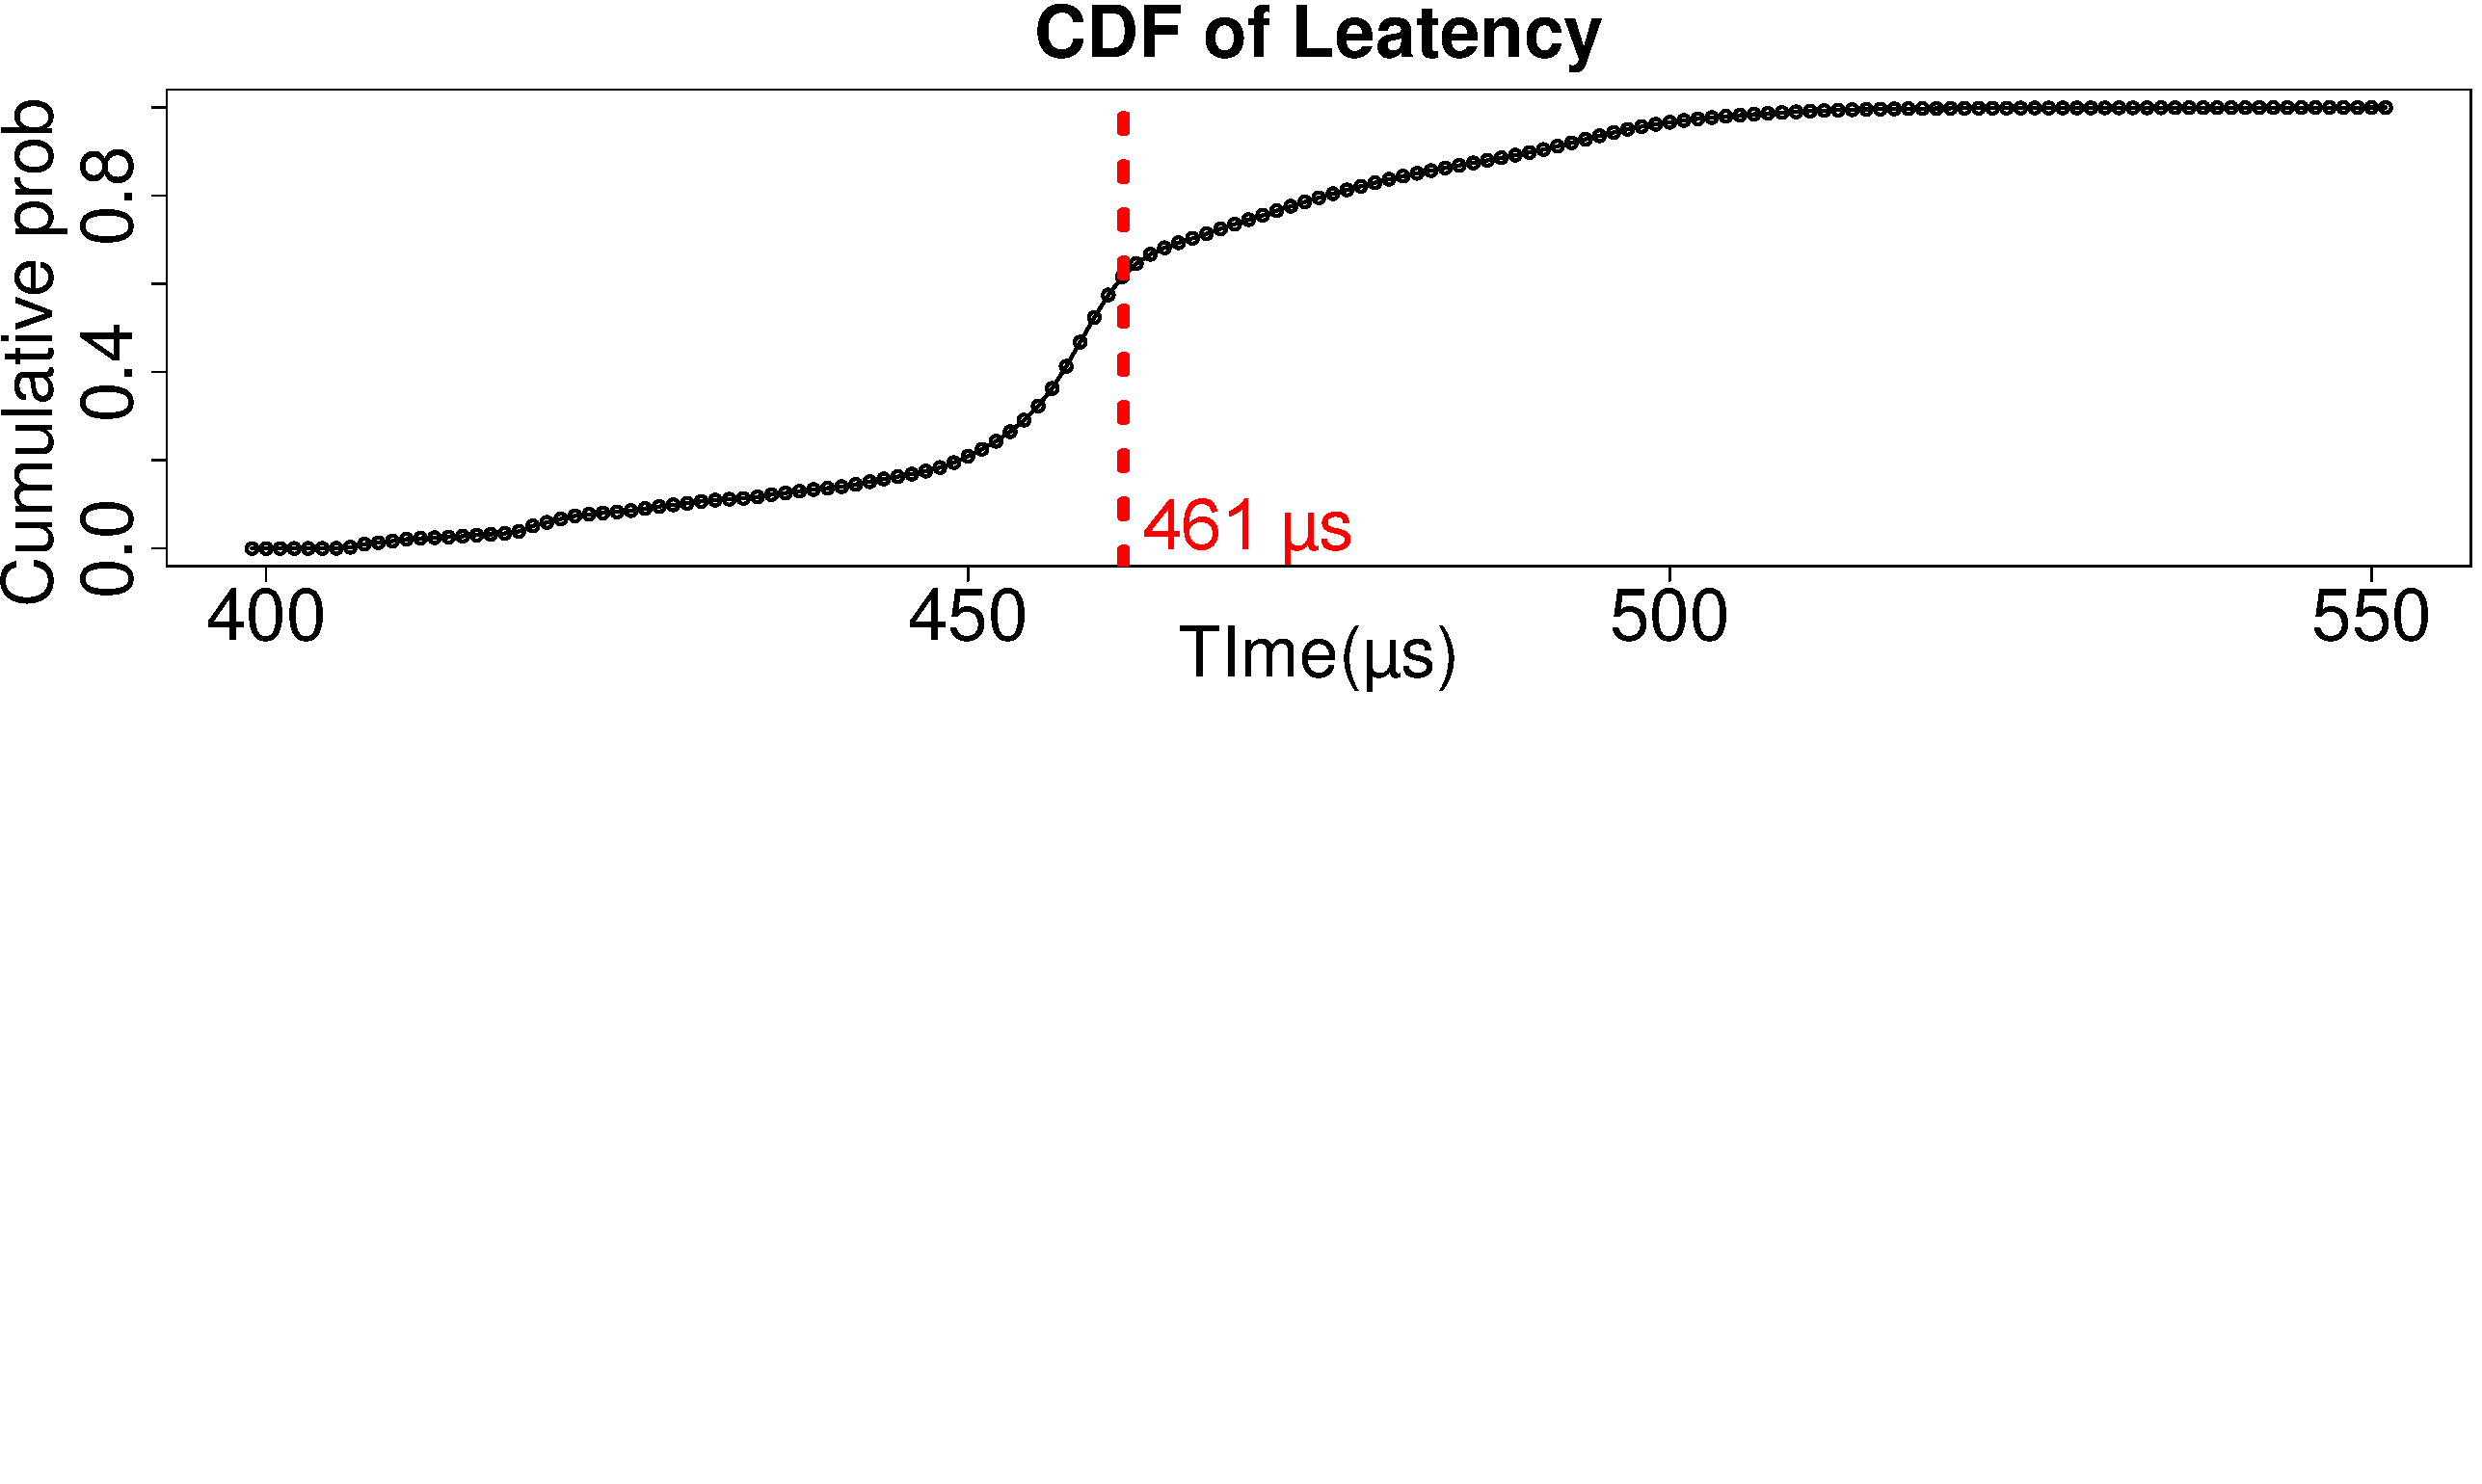
\includegraphics[trim={0 14cm 0 0}, clip, width=\linewidth]{data/graph/CDF_Latency1.pdf}
    %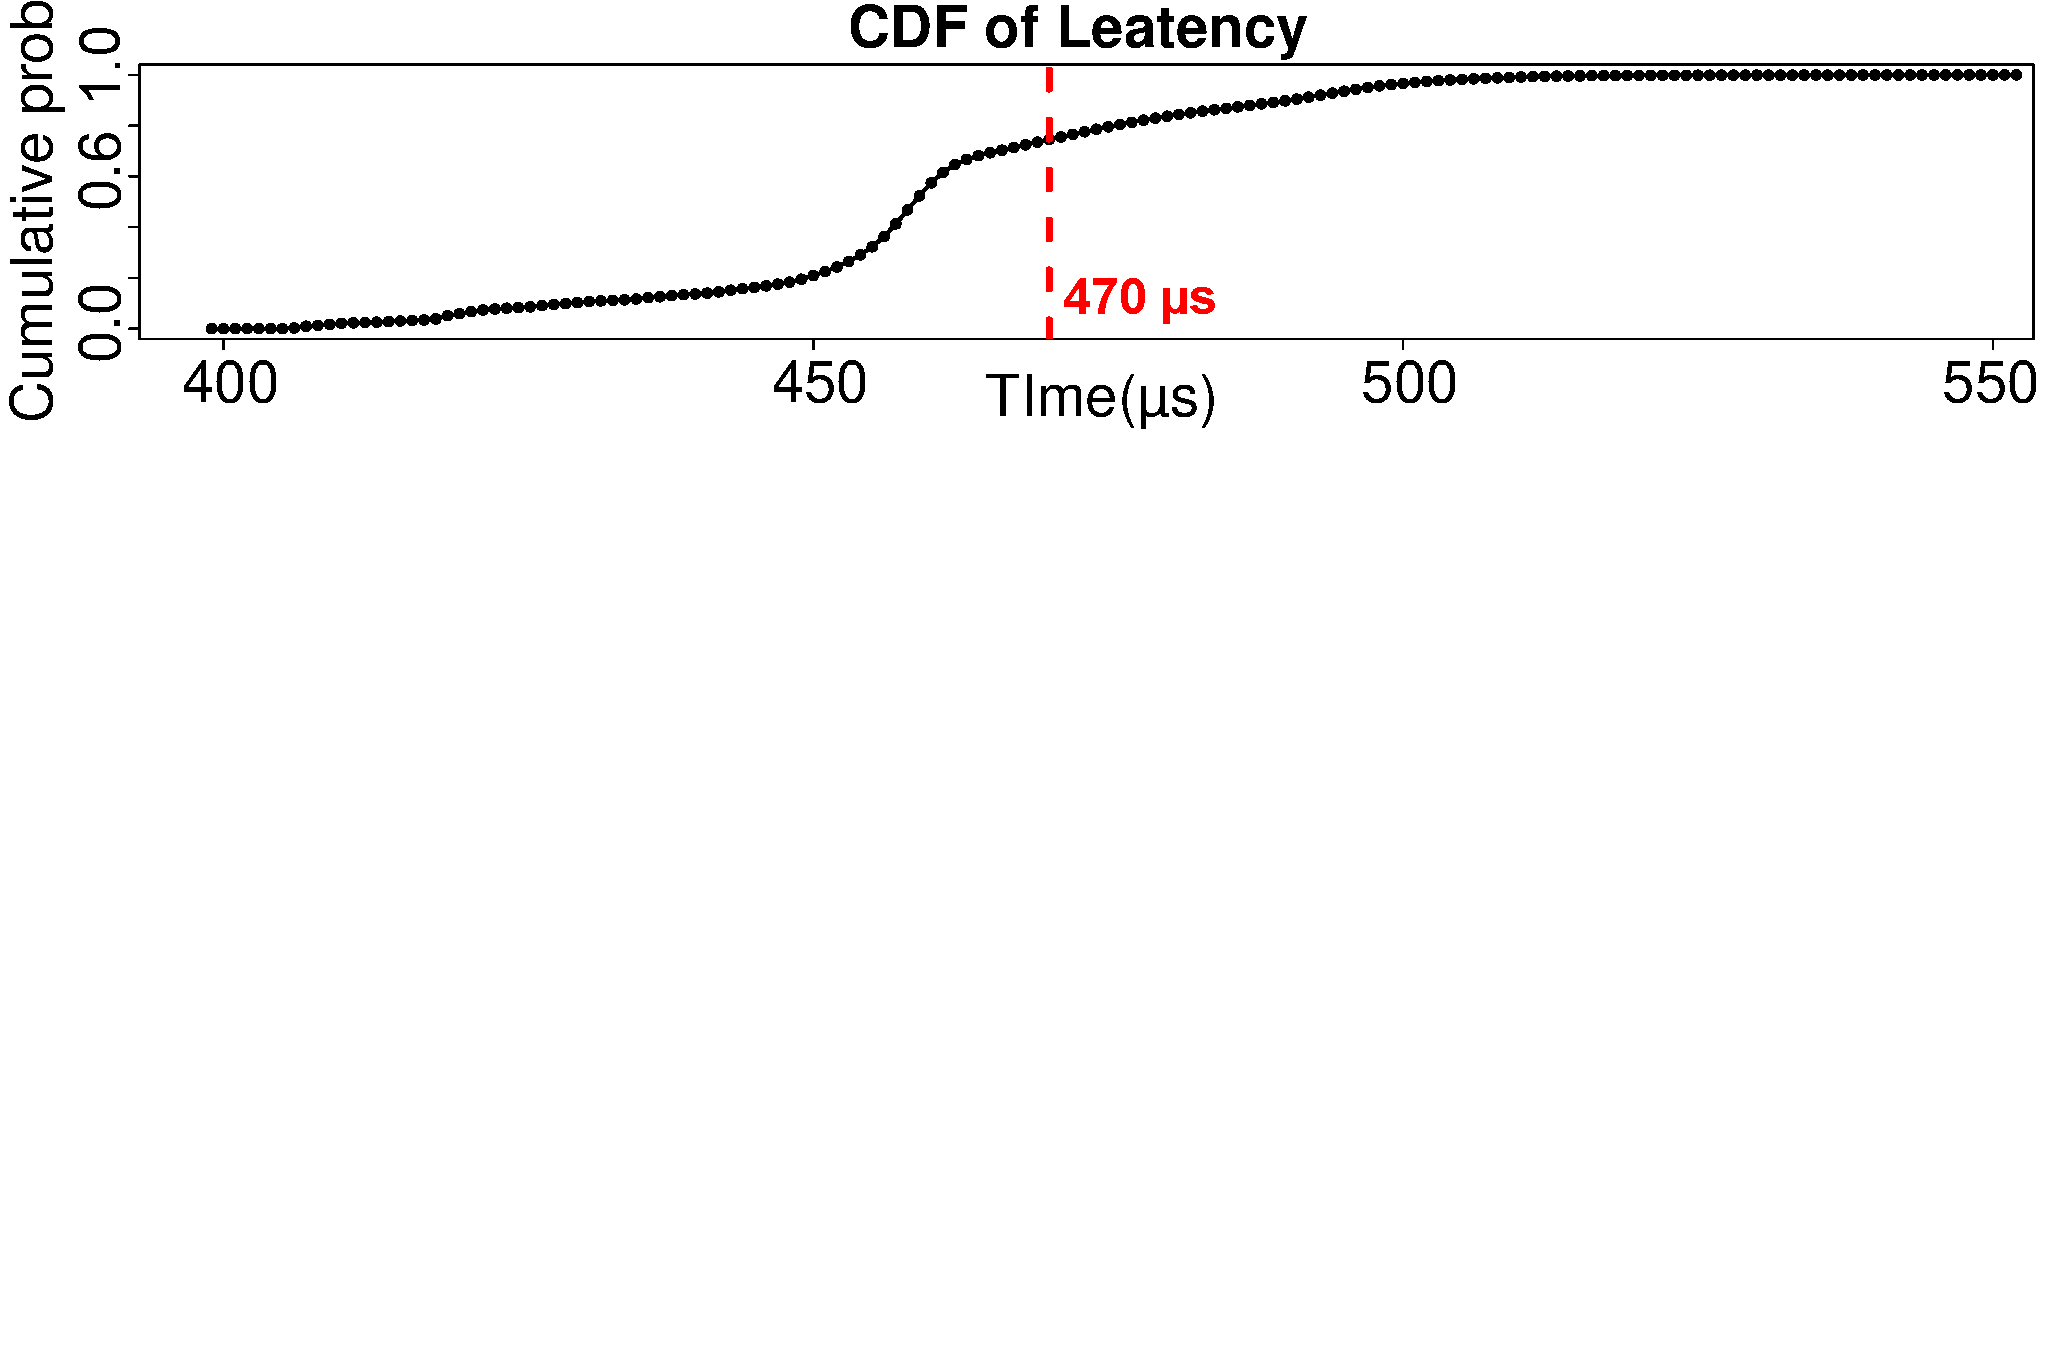
\includegraphics[trim={0 16cm 0 0}, clip,
    % width=\linewidth]{data/graph/CDF_Latency_new.pdf}
    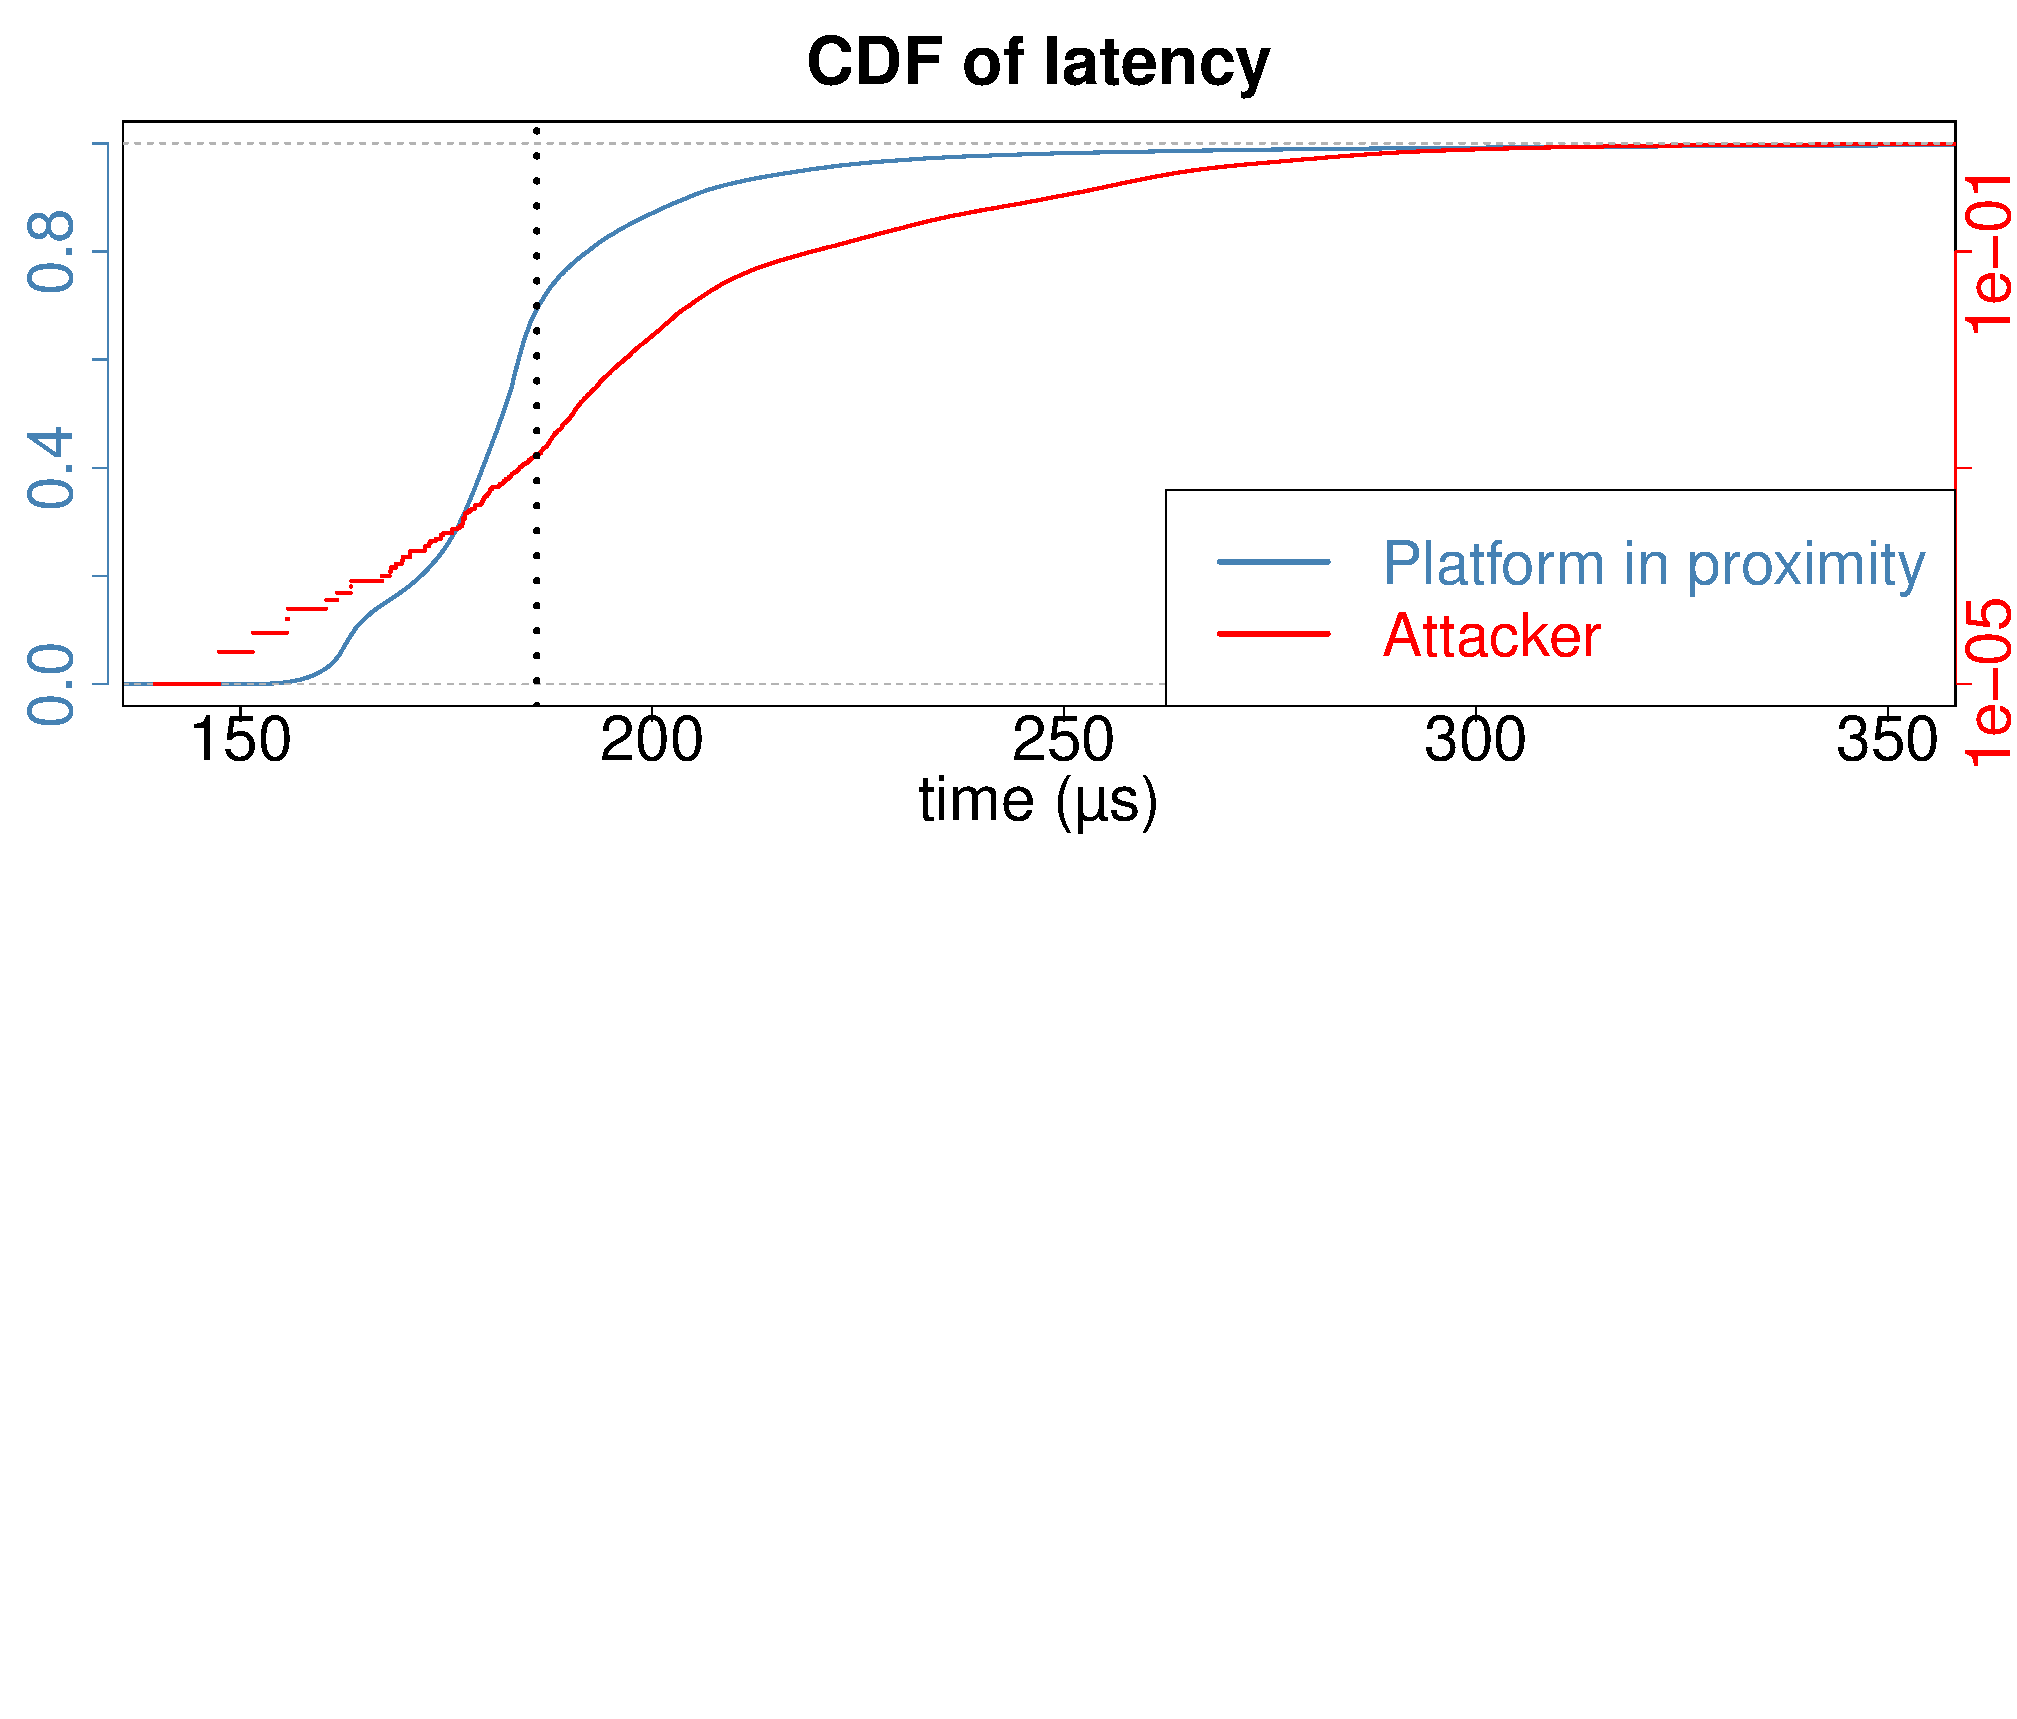
\includegraphics[trim={0 15cm 0 0}, clip, width=\linewidth]{data/fx3_data/CDF_N.pdf}
    \caption{Cumulative distribution function for latencies. We set the threshold \connect at 183 $\mu s$ which has a cumulative probability of $0.693$ in the experiment where no rerouting attack takes place with probability of $1.33\times10^{-4}$.}
    \vspace{-10pt}
    \label{fig:cdf}
\end{figure}


\myparagraph{1. Finding suitable threshold \connect.} Finding a suitable threshold \connect is a non-trivial task. A very low threshold requires a high number of the challenge-response rounds, since the protocol requires at least a fraction $k$ of the observed responses to be less or equal to \connect and a low threshold has very low cumulative probability value in the latency distribution (see Figure~\ref{fig:cdf}). Conversely, a very high threshold value enables some latencies measured during an attack to be classified as legitimate replies, hence increasing the chances of the attacker to break the proximity verification. To address this challenge, we perform a trial over multiple threshold candidates to evaluate their viability.


Figure~\ref{graph:diffTh} shows the legitimate success probability $P_{legit}$ for different number of rounds ($n\in\{10,20,50,100\}$). We iterate through multiple threshold times (\connect$\in\{183\mu s,184\mu s,185\mu s, 186\mu s, 189\mu s\}$), and $186\mu s$ provides high success ratio for different values of $k$ ($P_{legit}=0.9\{7\}77$ $(n=50)$ and $P_{legit}=0.9\{15\}29\ (n=100)$), where $0.9\{n\}x$ denotes $0.n$-times $9$ followed by $x$.

We test \connect up until $186 \mu s$ because as can be observed in Figure~\ref{graph:instatAttackerHisto} for these values we observe extremely small occurrences ($1.33\times10^{-3}$) of latency responses during an attacking scenario. It is possible to increment the latency further to improve the success probability, but doing so will start increasing the probability for the attacker as well. 
%
After that, we estimate that any latency value less than or equals to the threshold \connect appears with the cumulative probability of $p_{\mathcal{H}} = \Pr[144\leq x \leq 186] = \sum_{i=144}^{186}\Pr[x=i] = 0.693$ (where $144\ \mu s$ is the smallest latency experienced).
%
\iffalse
%this is no longer necessary
Using the standard error of the mean, we estimated the error in our model, which is approximately $p_e=1/(2\sqrt{\mathcal{N}})$~\footnote{Hoeffding's inequality~\cite{Hoeffding} describes that one needs at least $\frac{log(2/\alpha)}{2t^2}$ samples to acquire $(1-\alpha)$-confidence interval $E(\bar{X})\pm t$, we set $1-\alpha=95\%$.} where $\mathcal{N}$ denotes the number of samples drawn in our experiment.
We have around $\mathcal{N}=27$ million samples to construct the distribution. This makes the sampling error probability $p_e \approx 1.06\times10^{-4}$.
%
The attacker's success probability $p_\mathcal{A}$ for a single round is simply the sampling error, i.e., $p_\mathcal{A} = p_e = 1.06\times10^{-4}$ due to the standard error of the mean as in our experiment we encounter zero samples within 461 $\mu s$ for attack distribution. The legitimate enclave's success probability $p_\mathcal{H}$ for a single round is the cumulative probability above, i.e.,  $p_\mathcal{H} = p_c = 0.6461$, as can be seen from Figure~\ref{fig:cdf}.
\fi

The attacker's success probability for a single round is the cumulative probability sampled from the attacker's distribution (the grey histogram in Figure~\ref{graph:instatAttackerHisto}) $p_\mathcal{A} = \Pr[x \leq 186] = \sum_{i=160}^{183}\Pr[x=i] = 1.33 \times 10^{-4}$.


Now, for both cases (simulated attack and benign case) we can model the complete challenge-response protocol of $n$ rounds as a Bernoulli's trial where we look for at least $kn$ responses within $186\ \mu s$ out of $n$. We can write this cumulative probability as a binomial distribution:
%

\begin{align*}
    \Pr[x \geq nk] = \sum_{i=nk}^n\binom{n}{i} (p)^{i}(1-p)^{n-i};~~\text{where}~ p \in \{p_\mathcal{H}, p_\mathcal{A}\}
\end{align*}
%  \vspace{-3px}


\newcommand{\roundCompCaption}{\textbf{Finding suitable fraction $k$.} The graph shows the legitimate enclave's success probability in an ideal scenario and the attacker's success probability in rerouting attack scenario with varying $k$.}

\begin{figure}[t]
  \centering
    %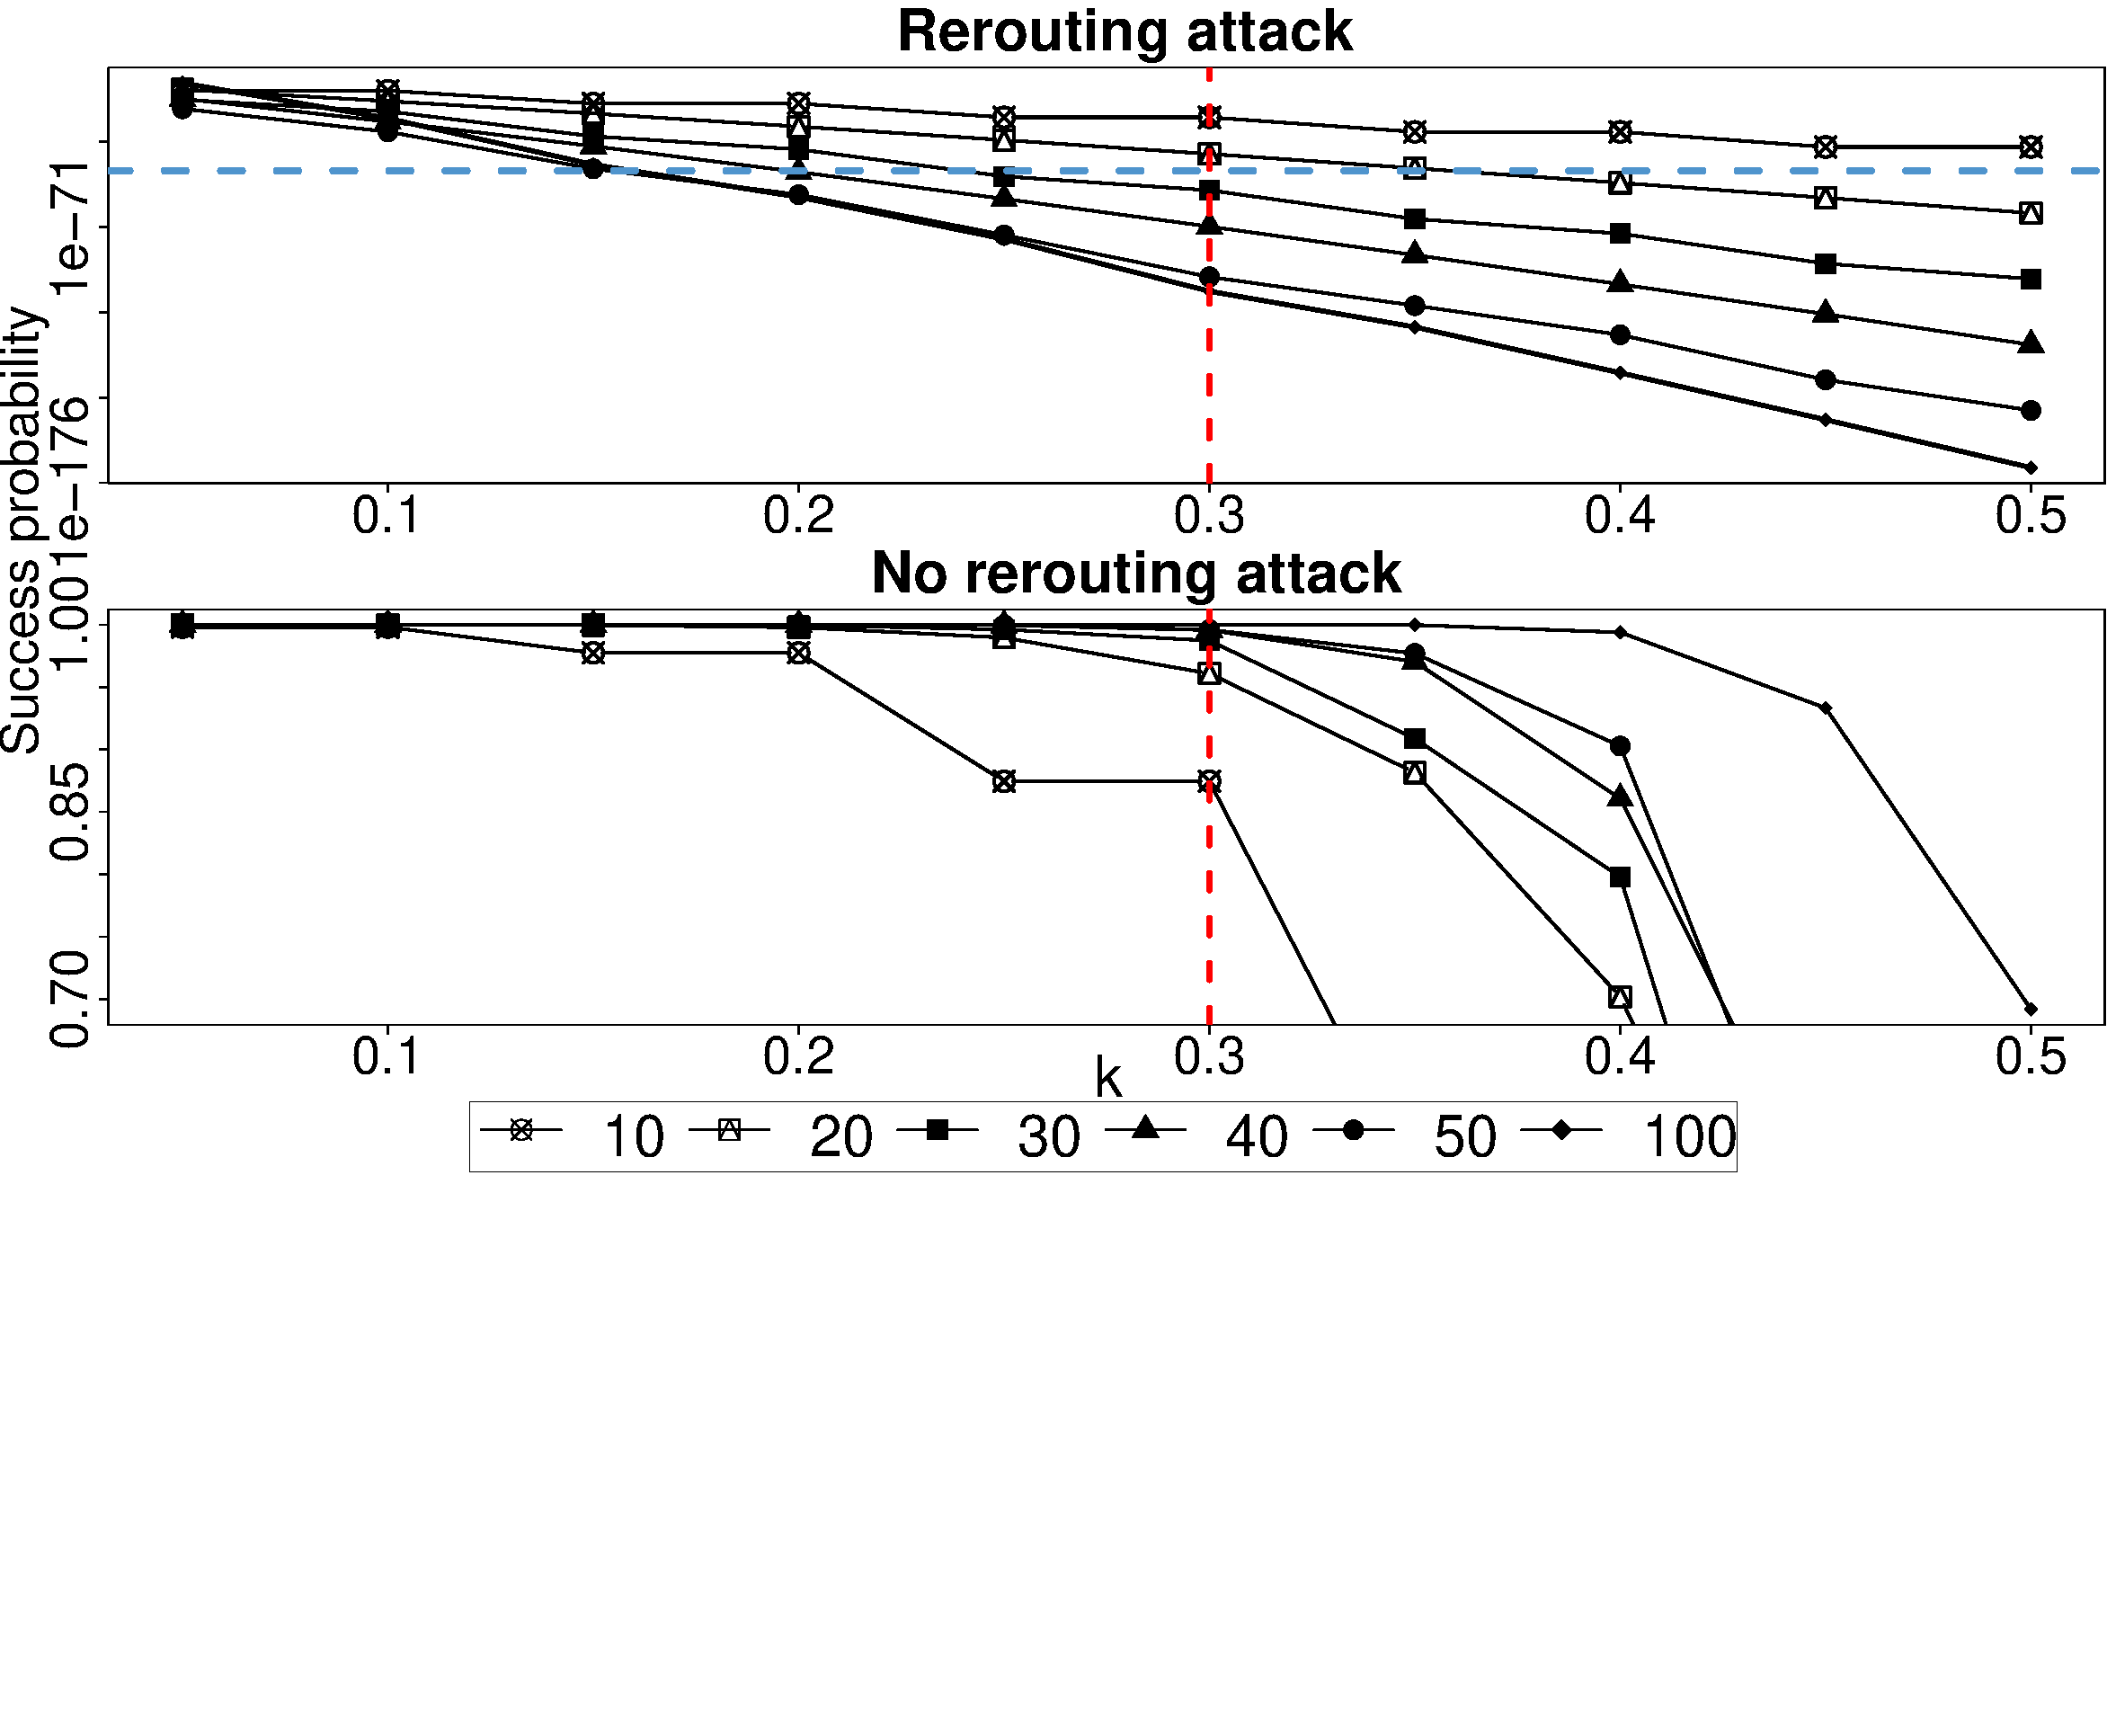
\includegraphics[trim={0 10.6cm 0 0}, clip, width=0.9\linewidth]{data/graph/round_comp_1.pdf}
    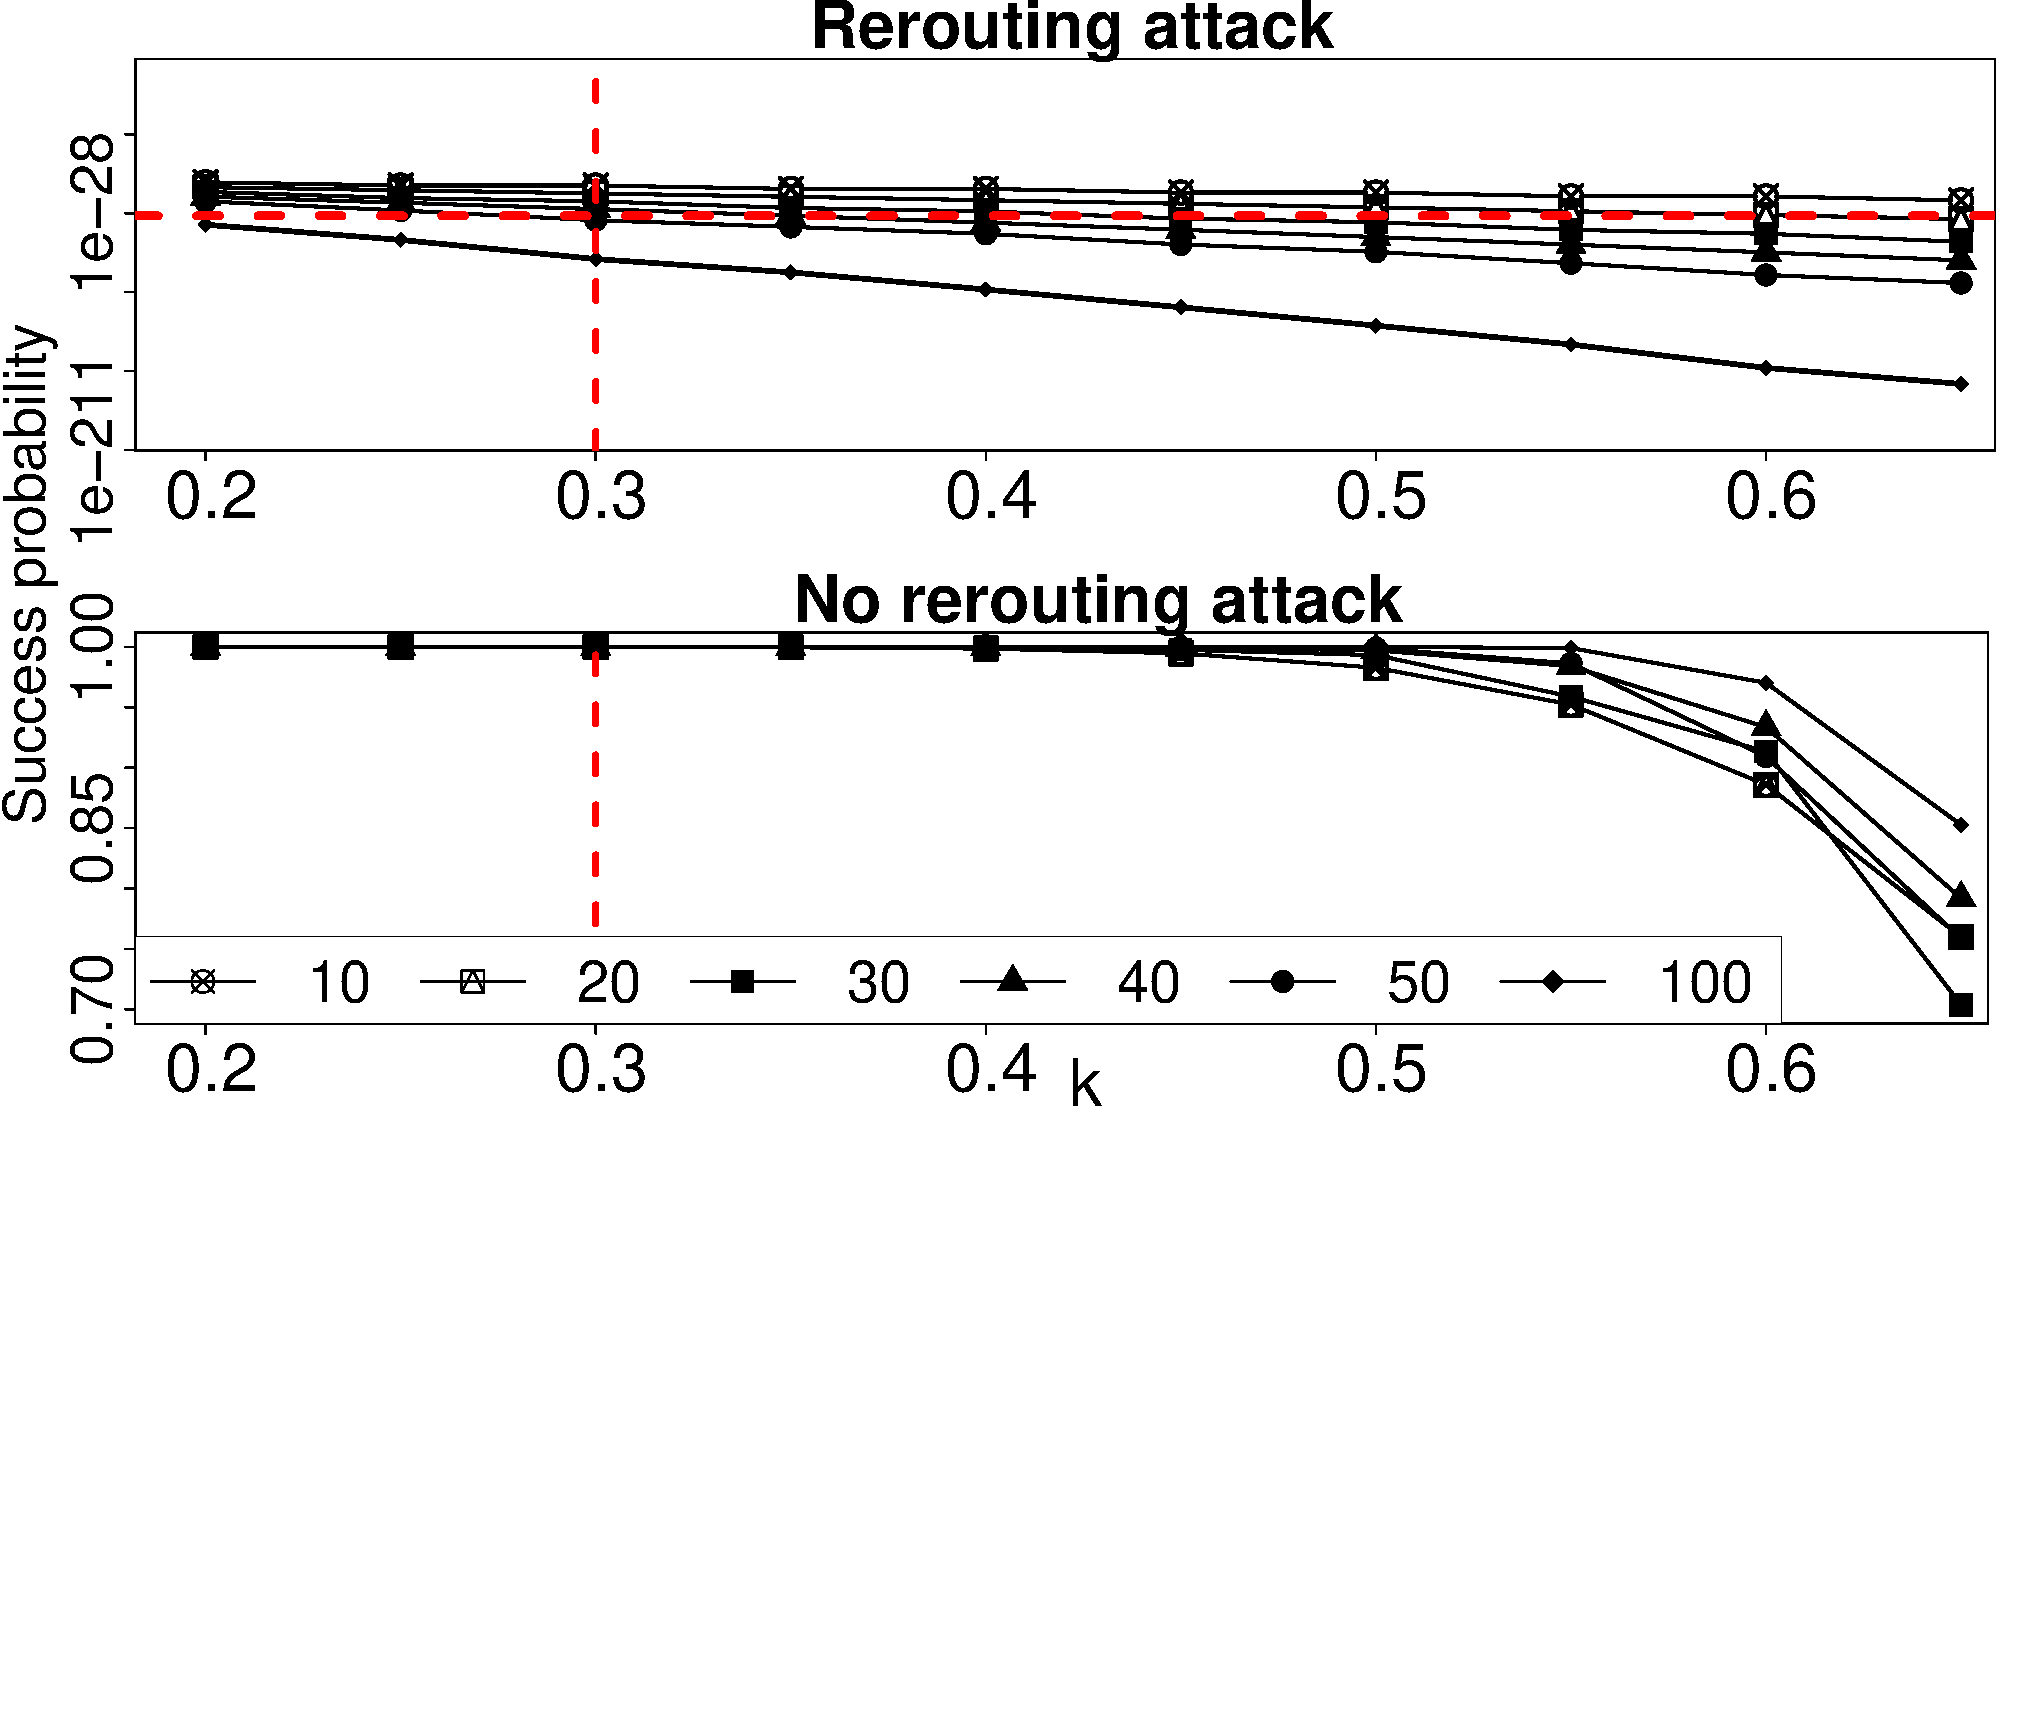
\includegraphics[trim={0 10cm 0 0}, clip, width=\linewidth]{data/fx3_data/round_comp_new.pdf}
    \caption{\roundCompCaption}
    %\vspace{-5px}
    \label{graph:roundSuccess}
\end{figure}


\myparagraph{2. Choosing a suitable fraction $k$.} The next step of the evaluation is to find a suitable fraction $k$ based on the threshold time \connect. Note that both the success probability of the attacker and the legitimate enclave is calculated as the cumulative probability from a binomial distribution (from $nk$ to $n$). Hence, we require to choose a suitable value of $k$ that maximizes $P_{legit}$ while minimizing $P_{adv}$.

We calculate two graphs that are depicted in Figure~\ref{graph:roundSuccess} where the x-axis denotes $k$, and the y-axis denotes attacker's success probability $P_{adv}$ and legitimate success probability $P_{legit}$, respectively, while using \connect$=186 \mu s$. We observe a sharp decrease in the legitimate success probability at $k=0.3$. Hence, fix $k=0.3$ to achieve the maximum $P_{legit}$. Additionally, in the graph of attacker's success probability, the red horizontal line is placed at $10^{-30} \approx 2^{-100}$. Hence we propose to choose any round configuration bellow this horizontal line, where $n \geq 40$. With number of rounds set to $n=50$ and $k=0.3$, we have $P_{legit}=0.99999997$ and $P_{adv}=3.55\times 10^{-34}$. Similar result could be also observed in Figure~\ref{graph:roundSuccess} where the success probability of the legitimate enclave decreases significantly after $k=0.55$ for \connect$=186\mu s$.

%The x-axis of the graph shows the threshold $k$ that denotes that at least $nk$ challenge-response out of $n$ has to be less or equal to $470\ \mu s$. 
%The blue line in the upper graph denotes negligible success probability ($10^{-40}\approx 2^{-133}$) for the attacker.}

% in the scenario where the attacker's average network latency is $153\ \mu s$ using the \texttt{ping} flood mode.}

\myparagraph{3. Generalizing the number of rounds $n$.} Figure~\ref{graph:instatAttackerHisto} extends this analysis to the general number of challenge-response rounds spanning from $n=2$ to $100$. Here we compute the probability of attacker returning the reply within $186 \mu s$ for at least $k=0.3$ fraction of challenges. The y-axis denotes the attacker's success probability which diminishes overwhelmingly with the increasing number of challenges (keeping the fraction constant at $k=0.3$). 

%Notice that, by merely choosing a higher number of rounds, satisfying values for the legitimate and attacker's success probabilities can be achieved even in the case in which the attacker manages to optimize the kernel for minimum network latency. Hence, \name can distinguish legitimate enclave and the attacker despite the lower latency. As long as the network latency is not negligible even smaller attacker's latencies than we could measure can be protected against by employing a higher number of challenge-response rounds.


\subsection{Periodic Proximity Verification}
\label{sec:newResults:cont}

In Section~\ref{sec:evaluationL:continuousParameters} we outlined a three-step approach for finding suitable parameters for the periodic proximity verification that we use for revocation. Here, we provide further details on each of these steps.

\myparagraph{1. Finding suitable threshold \detach.} We set the threshold \detach to $205\ \mu s$. We choose this value as we experience very small samples from the timing distribution (refer to the `yellow' distribution Figure~\ref{graph:instatAttackerHisto}) where no rerouting attack takes place. While in the attacker's distribution, the cumulative probability of the response occurring between \connect and \detach is $Pr[$\connect$\leq \mathcal{L}_{A} \leq$\detach$]=\sum_{i=186}^{205}\Pr[\mathcal{L}_{A}=i]=3.2\times10^{-2}$. 
%We account for the experimental error in our model using the standard error of the mean as  $p_e \approx 1.06\times10^{-4}$. The value $p_e$ signifies that a legitimate enclave running on the platform in proximity may take more than 649 $\mu s$ to respond. 
Using \detach, we can now define the challenge response rounds in Figure~\ref{fig:slidingWindow} for a \emph{single round} as following:
%
\begin{align*}
\Pr[\mathcal{L}_{legit}\leq T_{con}]&=\Pr[legit\in\text{green}]=0.693\\
\Pr[T_{con}< \mathcal{L}_{legit}< T_{detach}]&=\Pr[legit\in\text{yellow}]= 0.208\\
\Pr[\mathcal{L}_{legit}\geq T_{detach}]&=\Pr[legit\in\text{red}]= 1.83\times10^{-3}\\
\Pr[\mathcal{L}_{A}\leq T_{con}]&=\Pr[A\in\text{green}]=1.33\times10^{-3}\\
\Pr[T_{con}< \mathcal{L}_{A}< T_{detach}]&=\Pr[A\in\text{yellow}]= 0.032\\
\Pr[\mathcal{L}_{A}\geq T_{detach}]&=\Pr[A\in\text{red}]= 0.966\\
\end{align*} 


\myparagraph{2. Finding suitable sliding window size $w$.} Sliding window size is analogous to that of the number of rounds $n$. We keep  the size of the sliding window as $w=n=50$ as it only requires the \device to remember the past $50$ interactions and achieve high probability for the legitimate enclave and negligible success probability for the attacker. Similar to the previous approach, only if $15$ out of $50$ ($k=0.3$) challenge-response round where responses are within $186\ \mu s$, \name yields success probabilities as the following:
%
\begin{align*}
 \Pr[A \in \text{success window}]&=P'_{adv} = P'_{fn}= 3.55\times 10^{-34}\\
 \Pr[A \in \text{failed window}]&=\Pr[A\in\text{red}]^2=0.933\\
 \Pr[legit \in \text{success window}]&=0.99999997\\
 \Pr[legit \in \text{failed window}]&=P'_{fp}=\Pr[legit\in\text{red}]^2=3.34\times10^{-6}
\end{align*}


%leading to false negative (\name ruled out attack in a case of an attack) for the legitimate enclave of $3.77\times10^{-6}$) for the ideal scenario (refer to Figure~\ref{graph:roundSuccess}).


The probability that a halt window event occurs for a legitimate \app running on the platform in proximity is $\Pr[legit\in\text{red}]\approx 7.09\times10^{-3}$. The \device halts all the data communication to the target platform until the next periodic proximity verification.

If two or more than two latencies $\geq 205\mu s$ (\detach) are received, the \device terminates the connection and revoke the platform. The downtime that can happen as a result of false positive during a connection of 10 years is around $2$ minutes.


\myparagraph{3. Finding suitable frequency $f$.} The frequency $f$ determines how fast the connection is terminated in case the \device device is detached. Note that the \device takes around $500$ $\mu s$ on average to issue a new random challenge in the legitimate case. Hence, by performing a round of the protocol as soon as the previous is over, we achieve the maximum attainable average frequency of $\sim2000$ rounds per second. We use this frequency as it consumes only $156.14$ KB ($2.4\times 10^{-3}$\% of the USB 3.0 channel capacity) and allows the communication channel to be halted on average after $200 \mu s$ of the start of a relay attack and terminated in $1000 \mu s$ or 1 $ms$.


% ================================================== %

\subsection{Additional Experimental Results}
\label{appendix:ex}

%In this appendix we provide results from additional experiments.

%We evaluated the consistency of measured latencies across different computing platforms. Figure~\ref{graph:sgxLatency} shows the frequency distribution of latencies across three SGX platforms and three \device devices. We conclude that measurements are consistent result across devices. The two Intel NUCs are few microseconds faster than the Dell Latitude laptop. Additionally, we evaluated the effect of two different \usb cable lengths (3m and 1m) and three different Ethernet cables (lengths of 1m, 7m, and 10m). Figure~\ref{graph:usbCableLength} shows (on the right) that the \usb cable has very small effect on the latency (around 10 $\mu s$ average difference). It also shows (on the left) no significant differences between the different Ethernet cable lengths. 

%Figure~\ref{fig:osci} shows the challenge-response timing trace that we captured from the oscilloscope.

\iffalse
\begin{figure}[t]
  \centering
    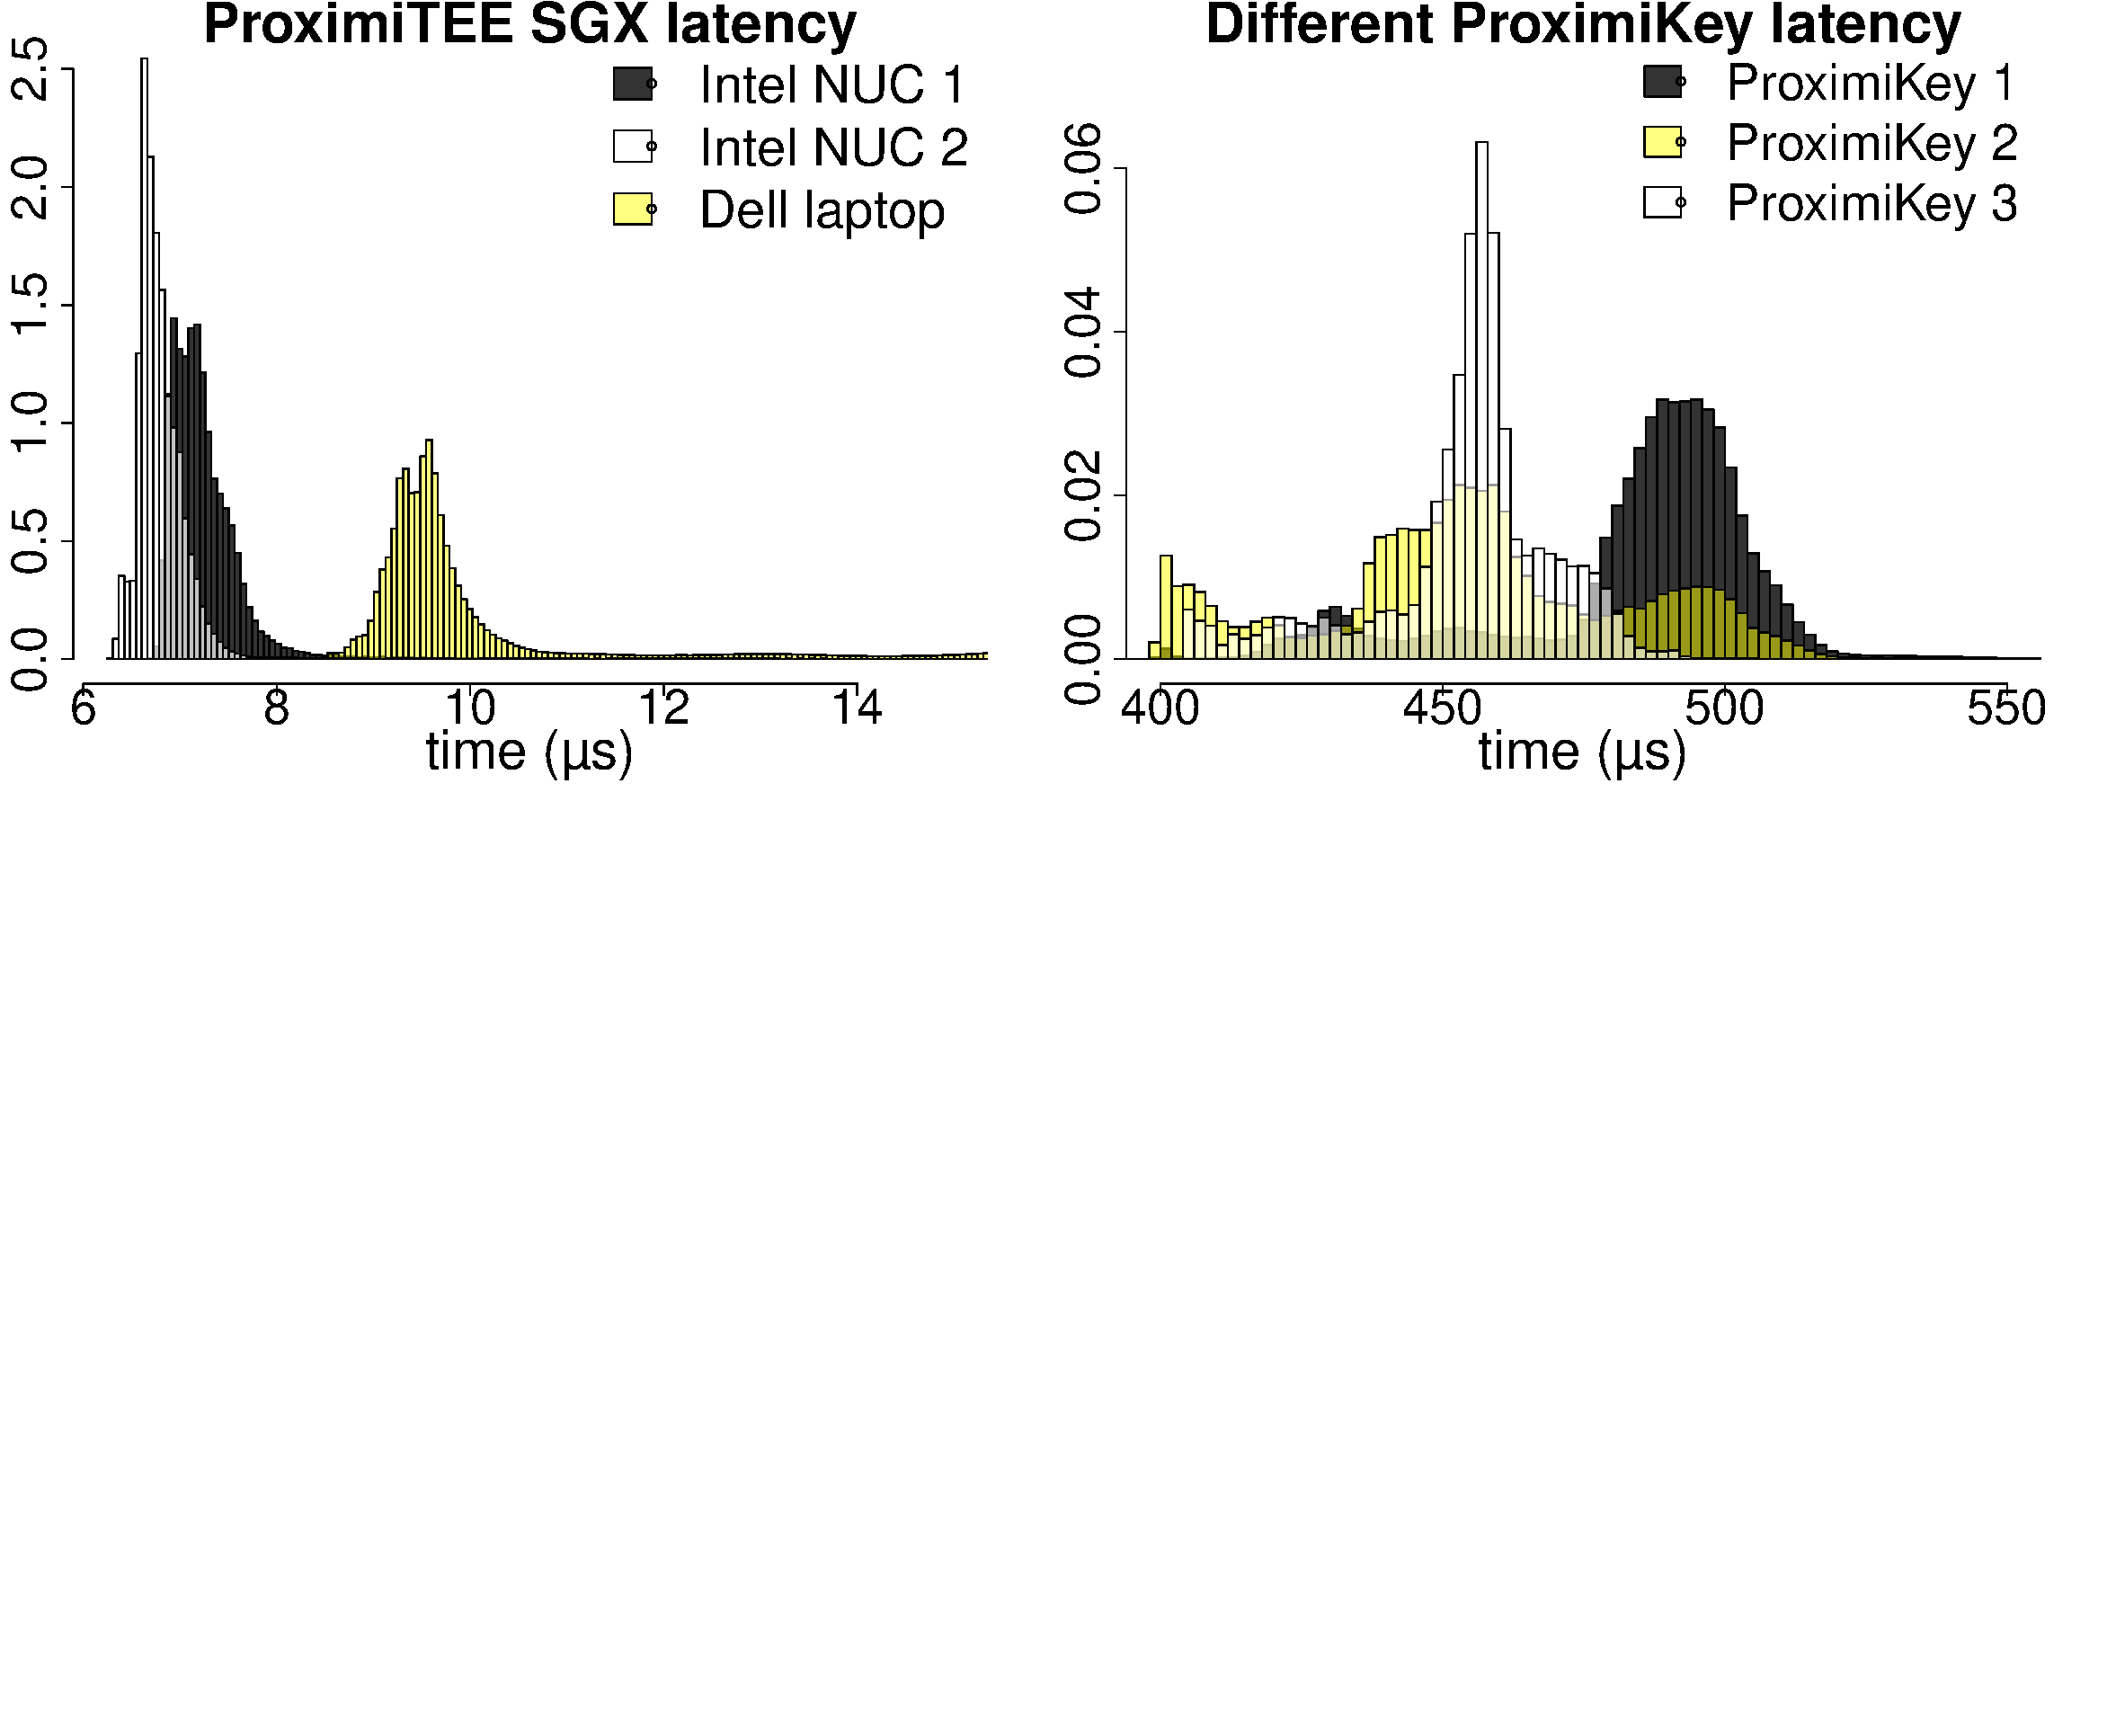
\includegraphics[trim={0 18cm 0 0}, clip, width=\linewidth]{data/graph/PlatformDevice_1.pdf}
    \caption{\textbf{Different target platforms/\device.} We evaluates latencies using three different SGX platforms. The Intel NUCs were few microseconds faster. Additionally, we evaluated latencies using three different Arduino boards. The latencies are consistent.}
    %\vspace{-17pt}
    \label{graph:sgxLatency}
\end{figure}
\fi

% \begin{figure}[h]
%   \centering
%     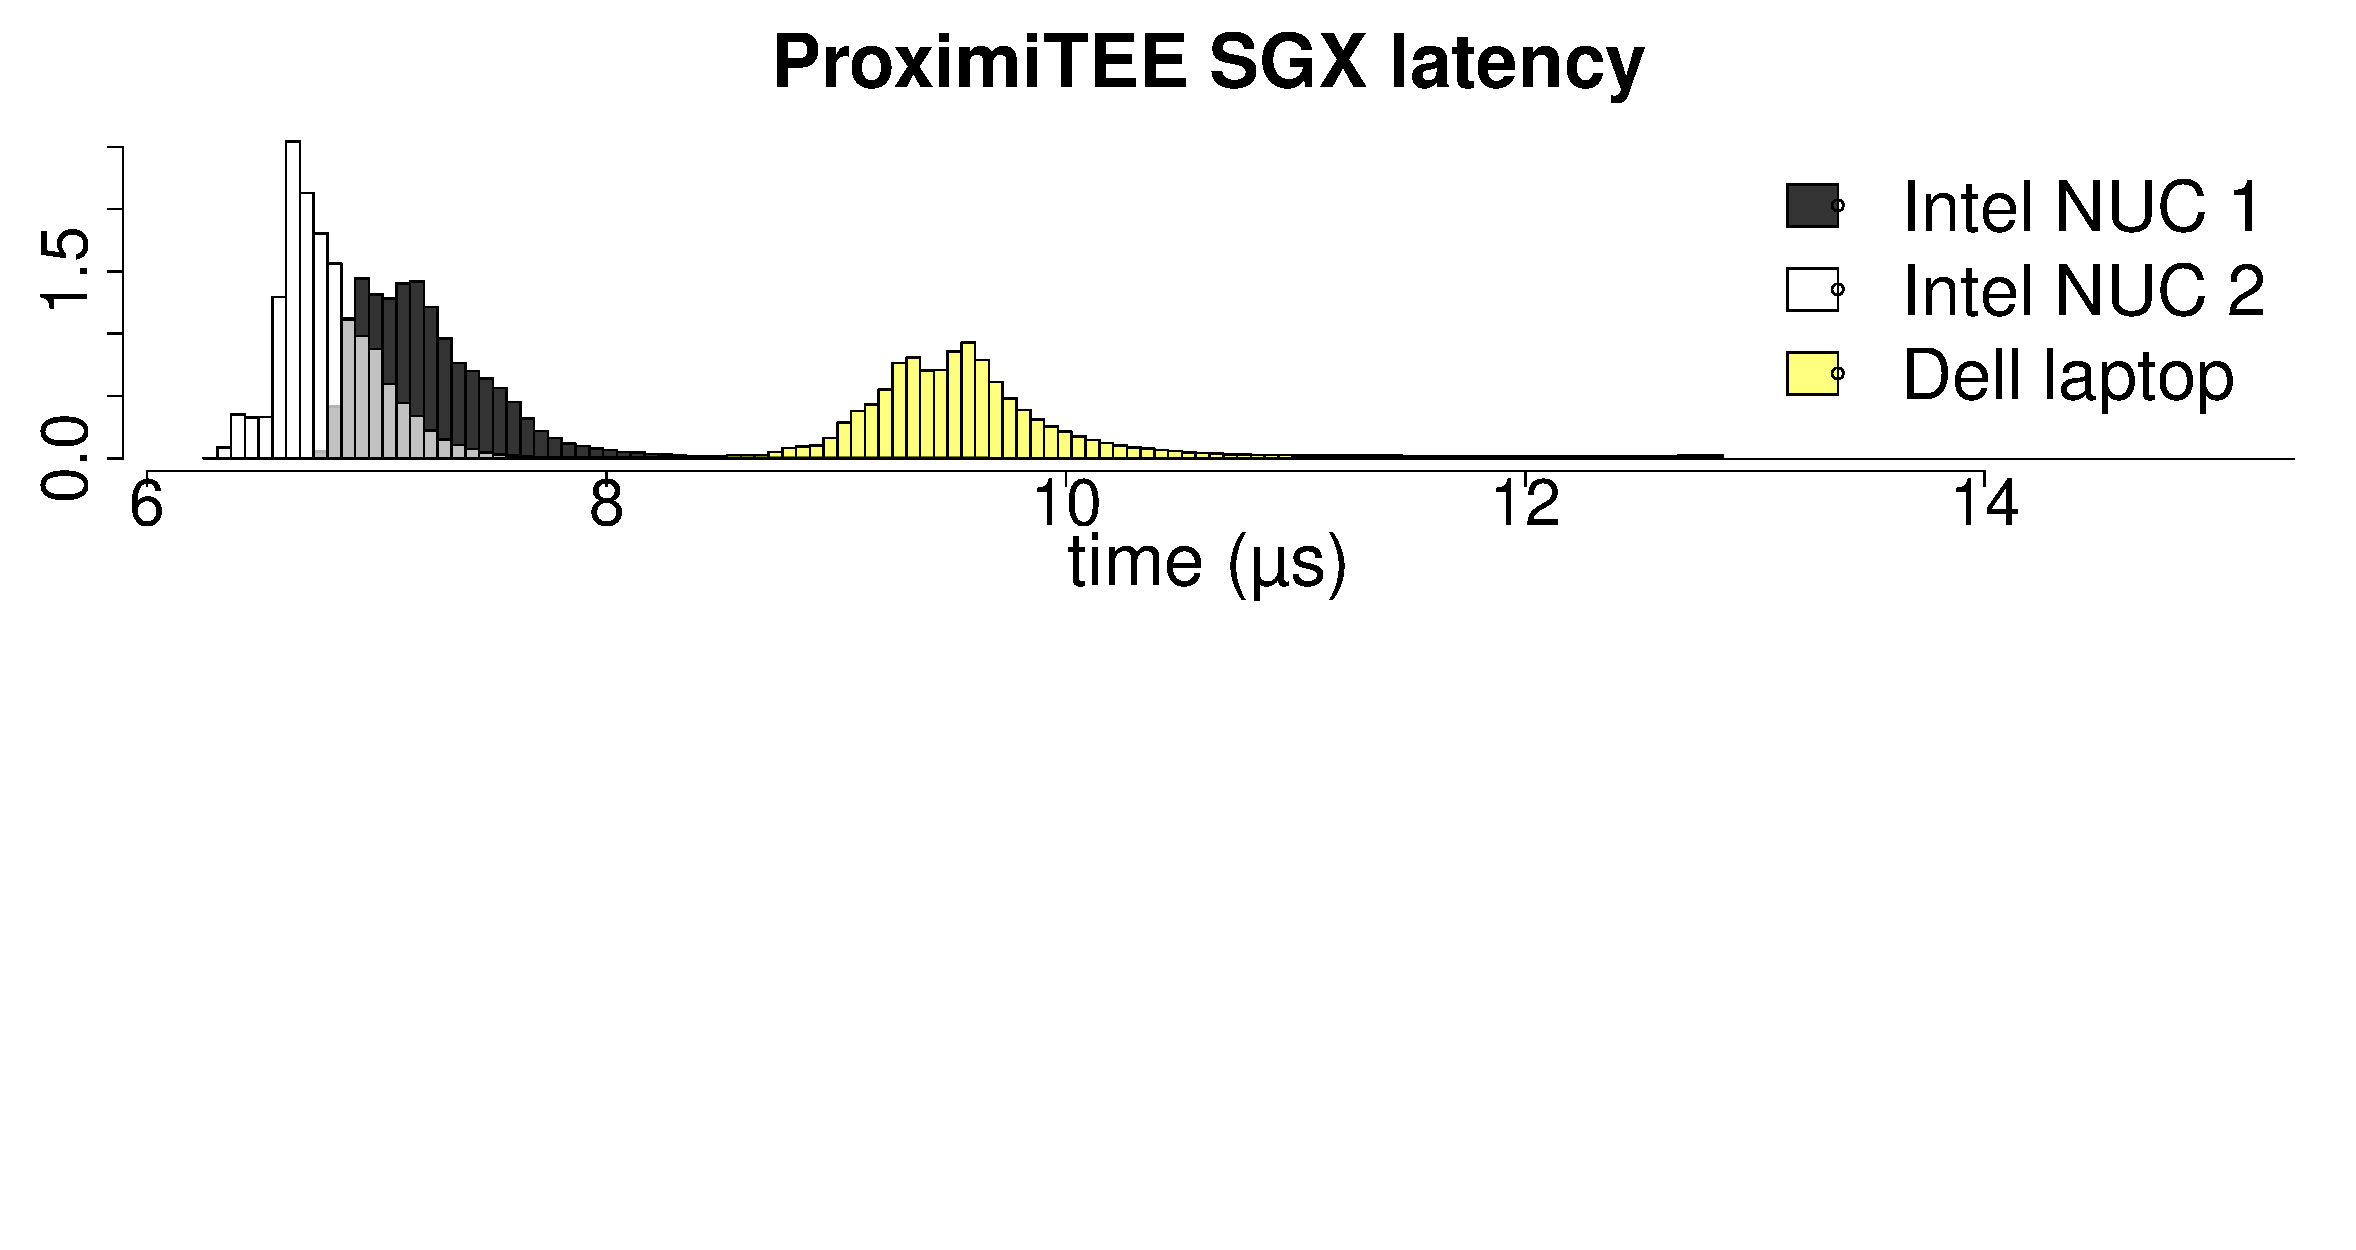
\includegraphics[trim={0 11cm 0 0}, clip, width=\linewidth]{data/graph/SGXLatency_1.pdf}
%     \caption{\textbf{Different target platforms.} We evaluates latencies using three different SGX platforms. The Intel NUCs were few microseconds faster.}\vspace{-15pt}
%     \label{graph:sgxLatency}
% \end{figure}
%
%  \begin{figure}[h]
%   \centering
%     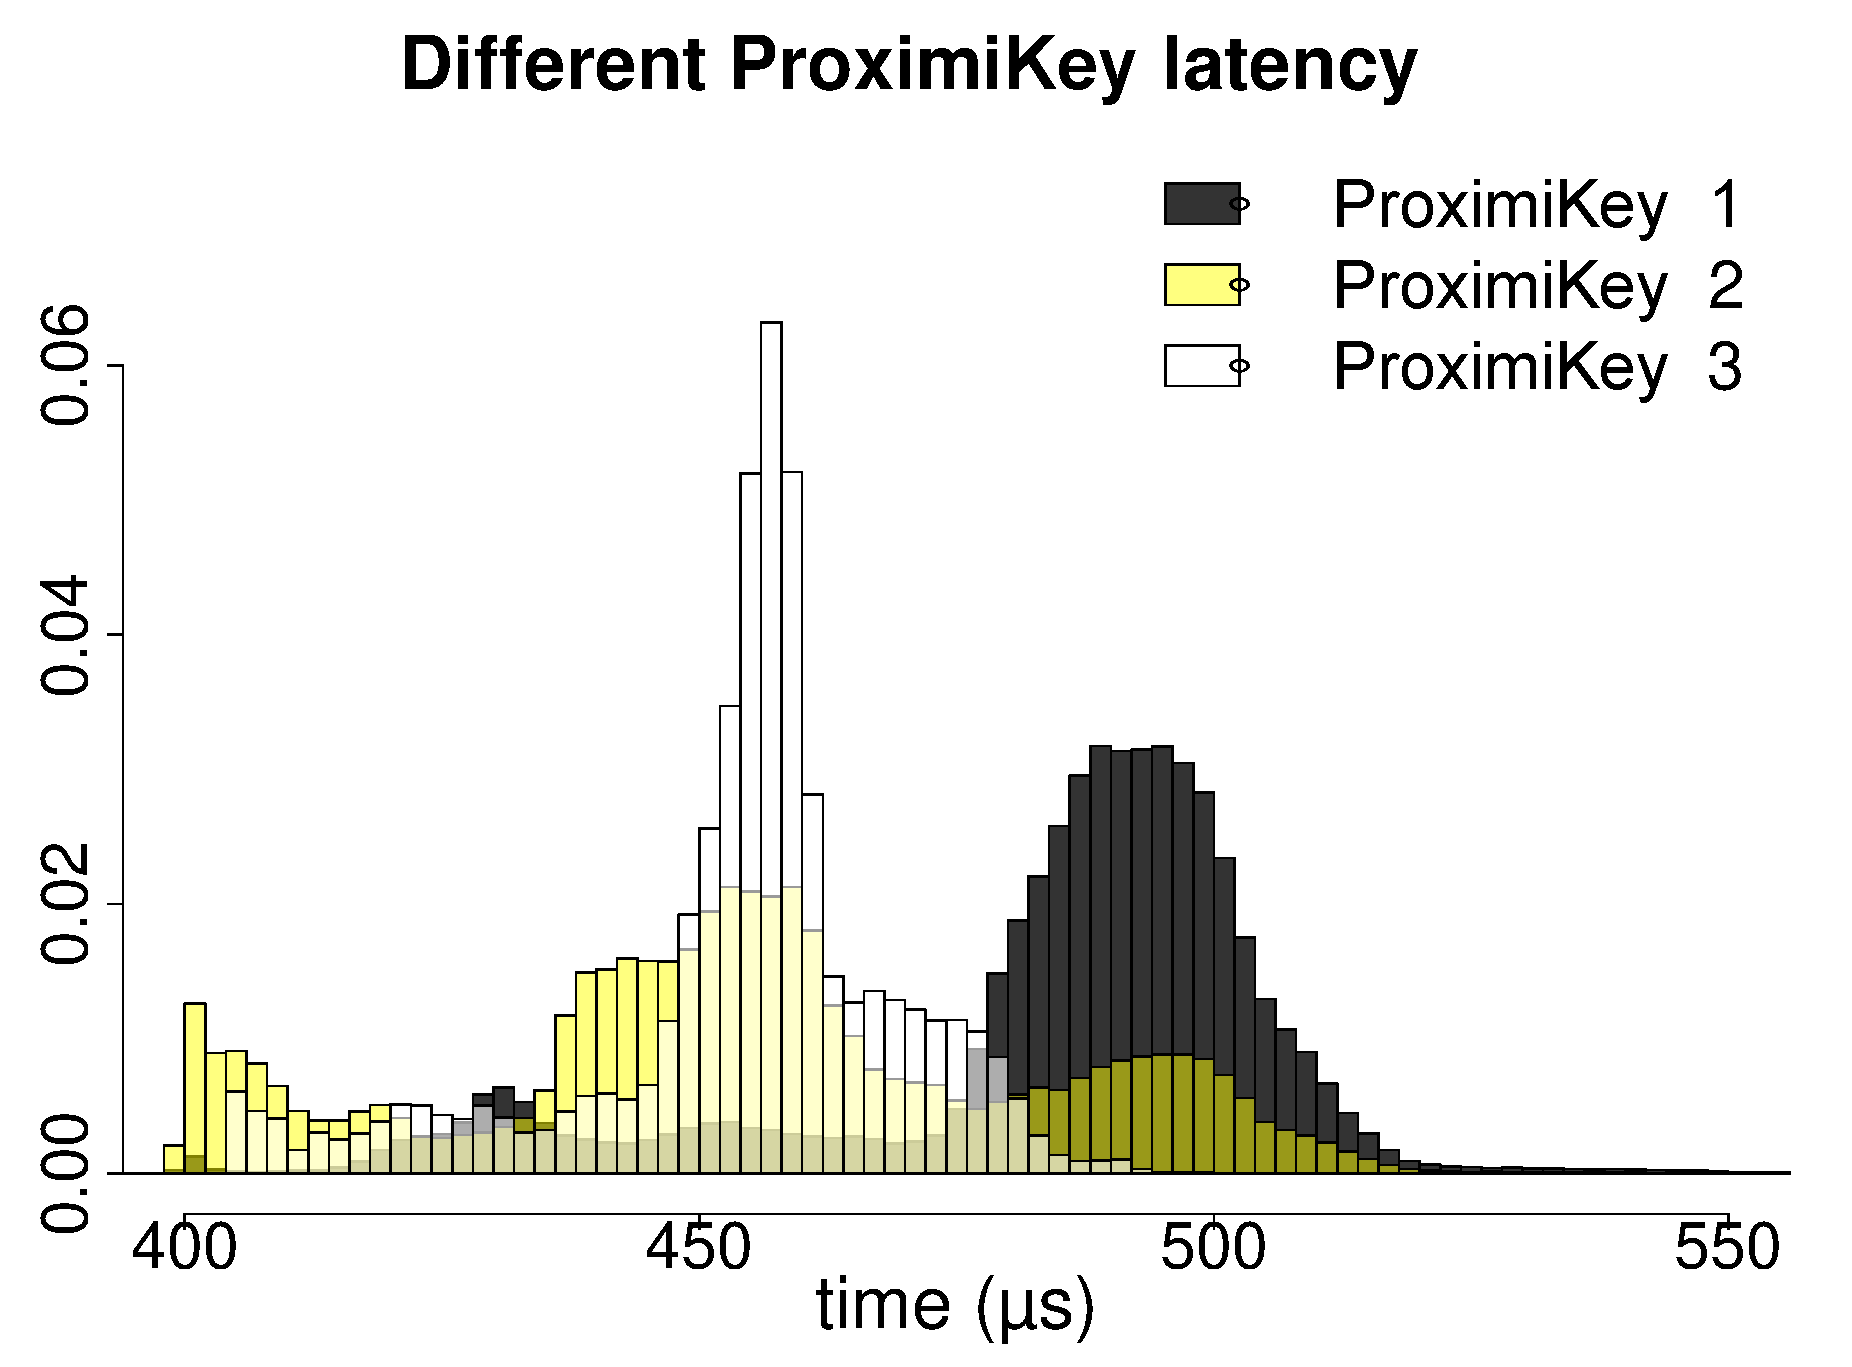
\includegraphics[trim={0 0 0 0}, clip, width=0.75\linewidth]{data/graph/DeviceLatency.pdf}
%     \caption{\textbf{Different embedded devices.} We evaluated latencies using three different Arduino boards. The latencies are consistent.}
%     \vspace{-20pt}
%     \label{graph:devices}
% \end{figure}

\iffalse
\begin{figure}[t]
  \centering
    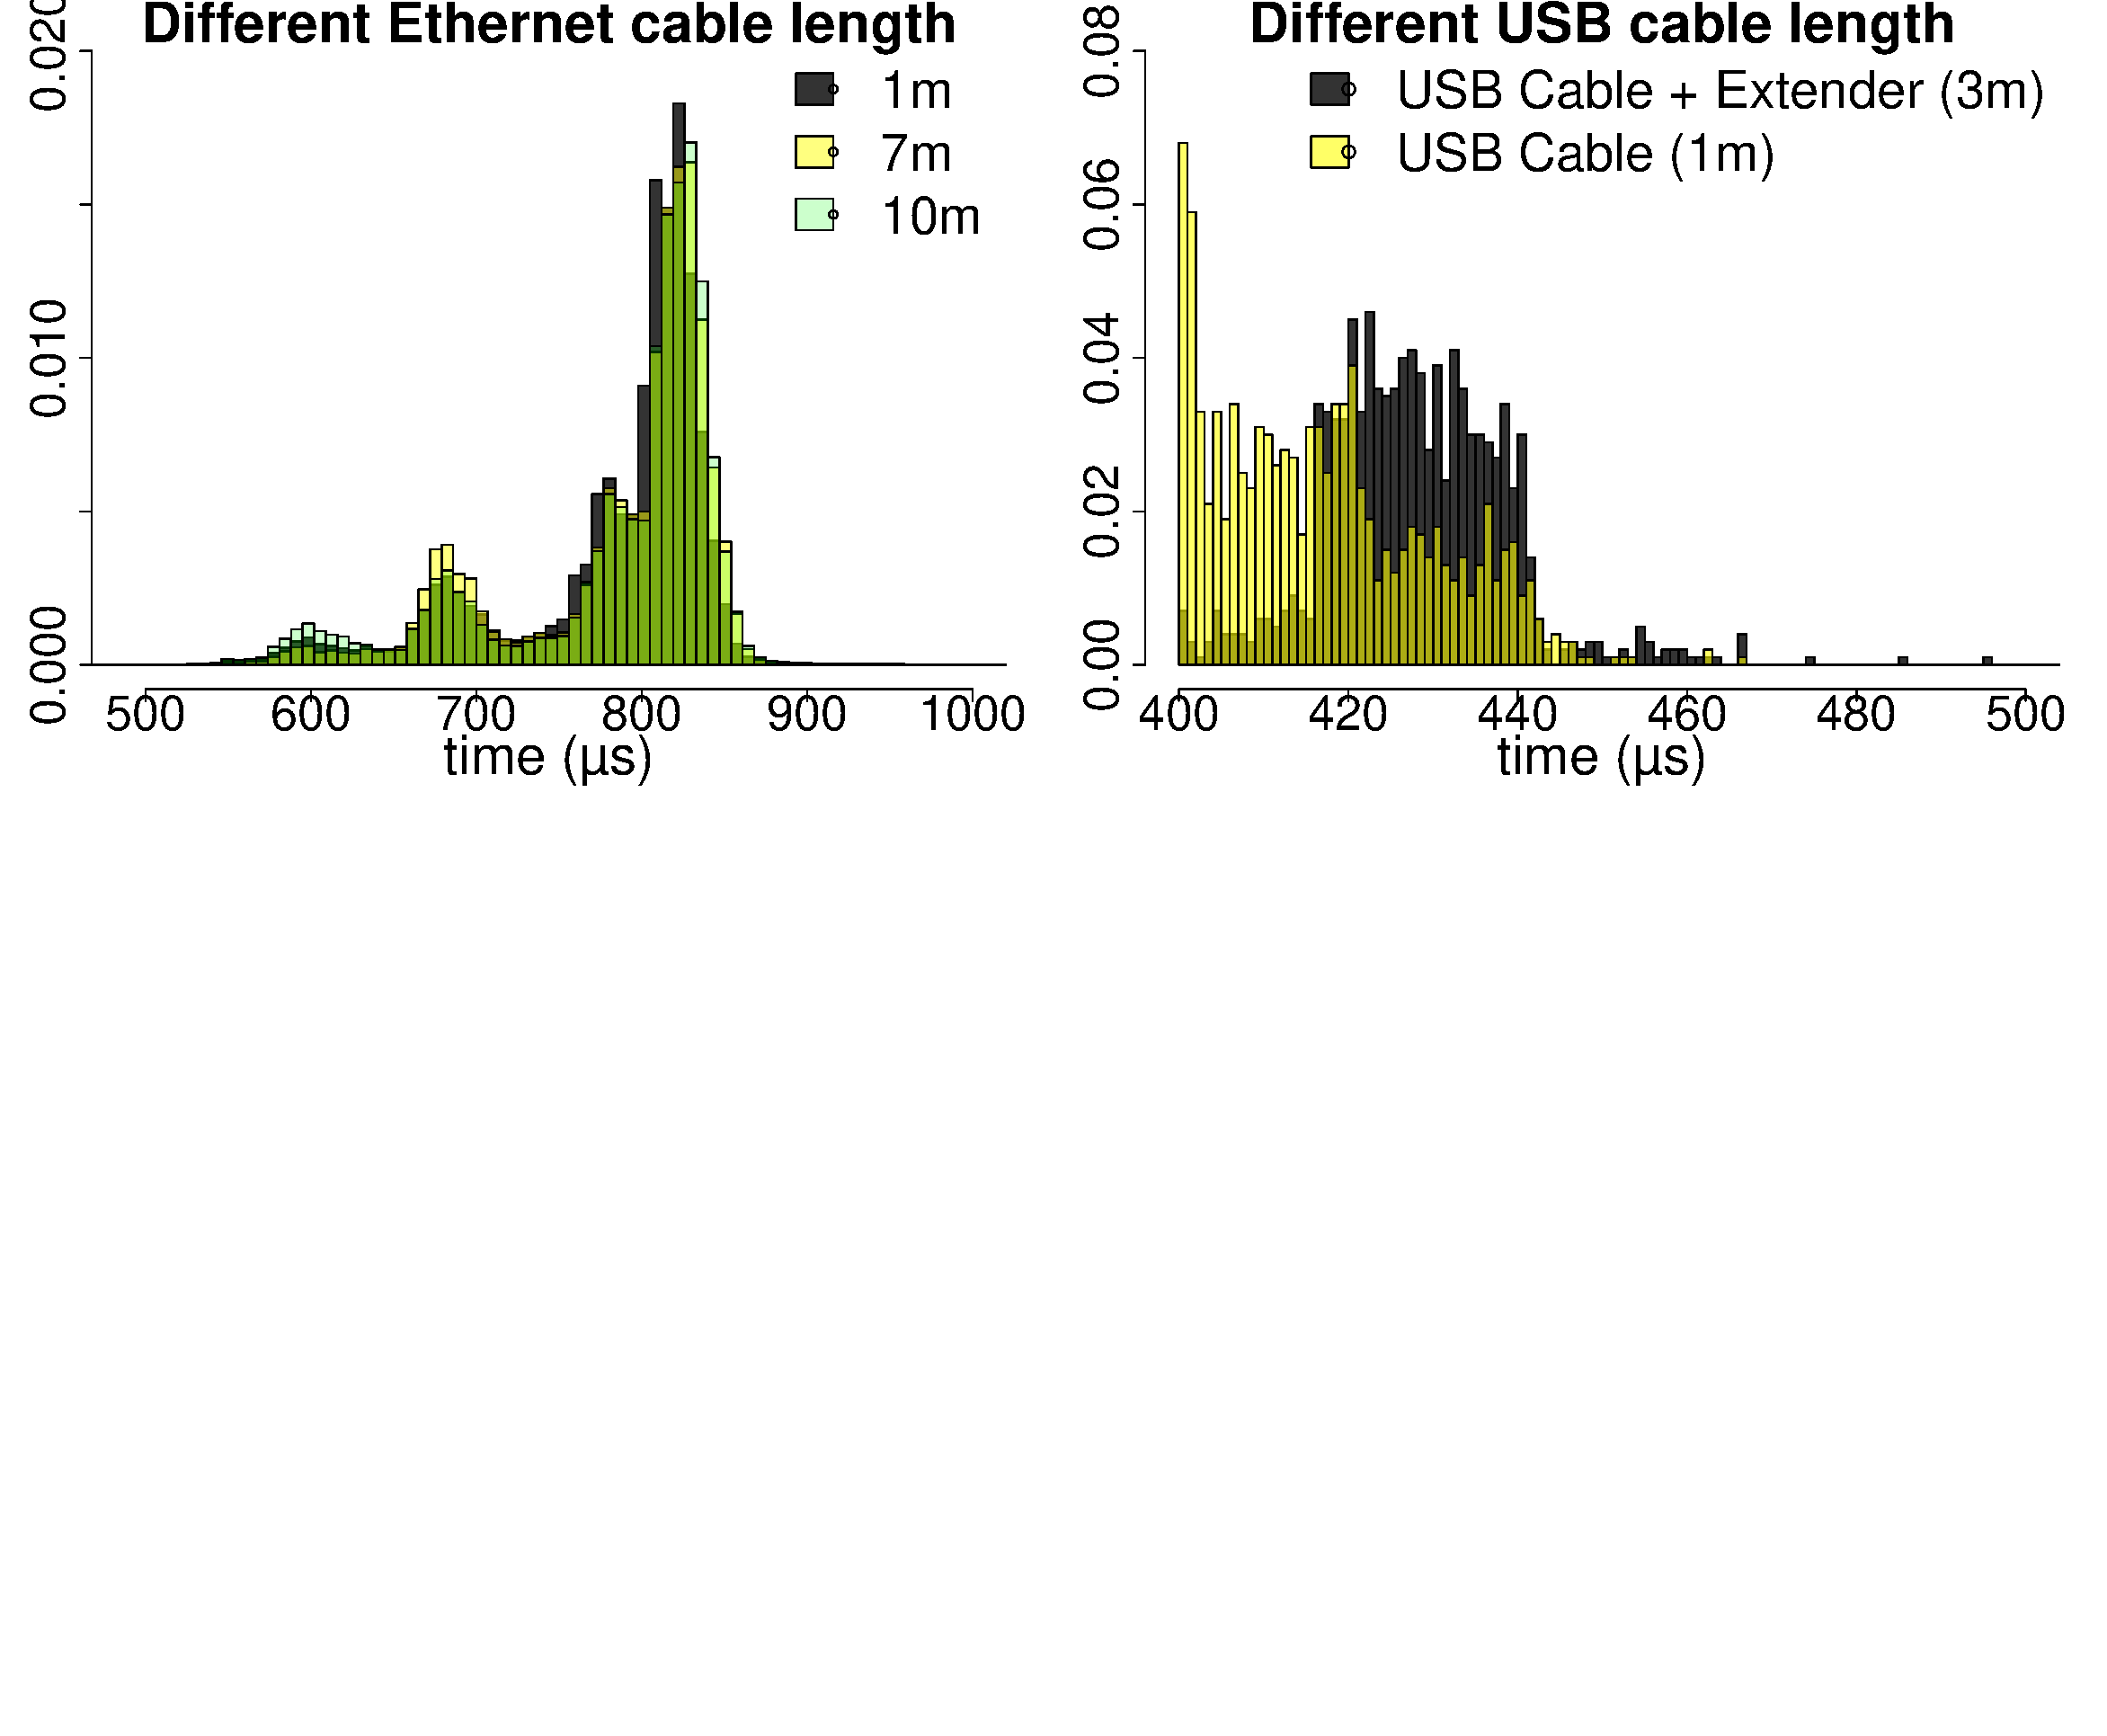
\includegraphics[trim={0 18cm 0 0}, clip, width=\linewidth]{data/graph/CombinedCable_1.pdf}
    \caption{\textbf{Different Ethernet/USB cables.} We evaluated latencies two different USB cables: one with an \usb cable (1m) and another with an \usb extender of length 2m attached. Additionally, we evaluated latencies using three different Ethernet cables (1, 7 and 10 m). Latencies are consistent. Note, that the latency is sampled in the experiment conducted with non-\texttt{ping} flood mode.}
    \label{graph:usbCableLength}
\end{figure}
\fi

\begin{figure}[t]
  \centering
    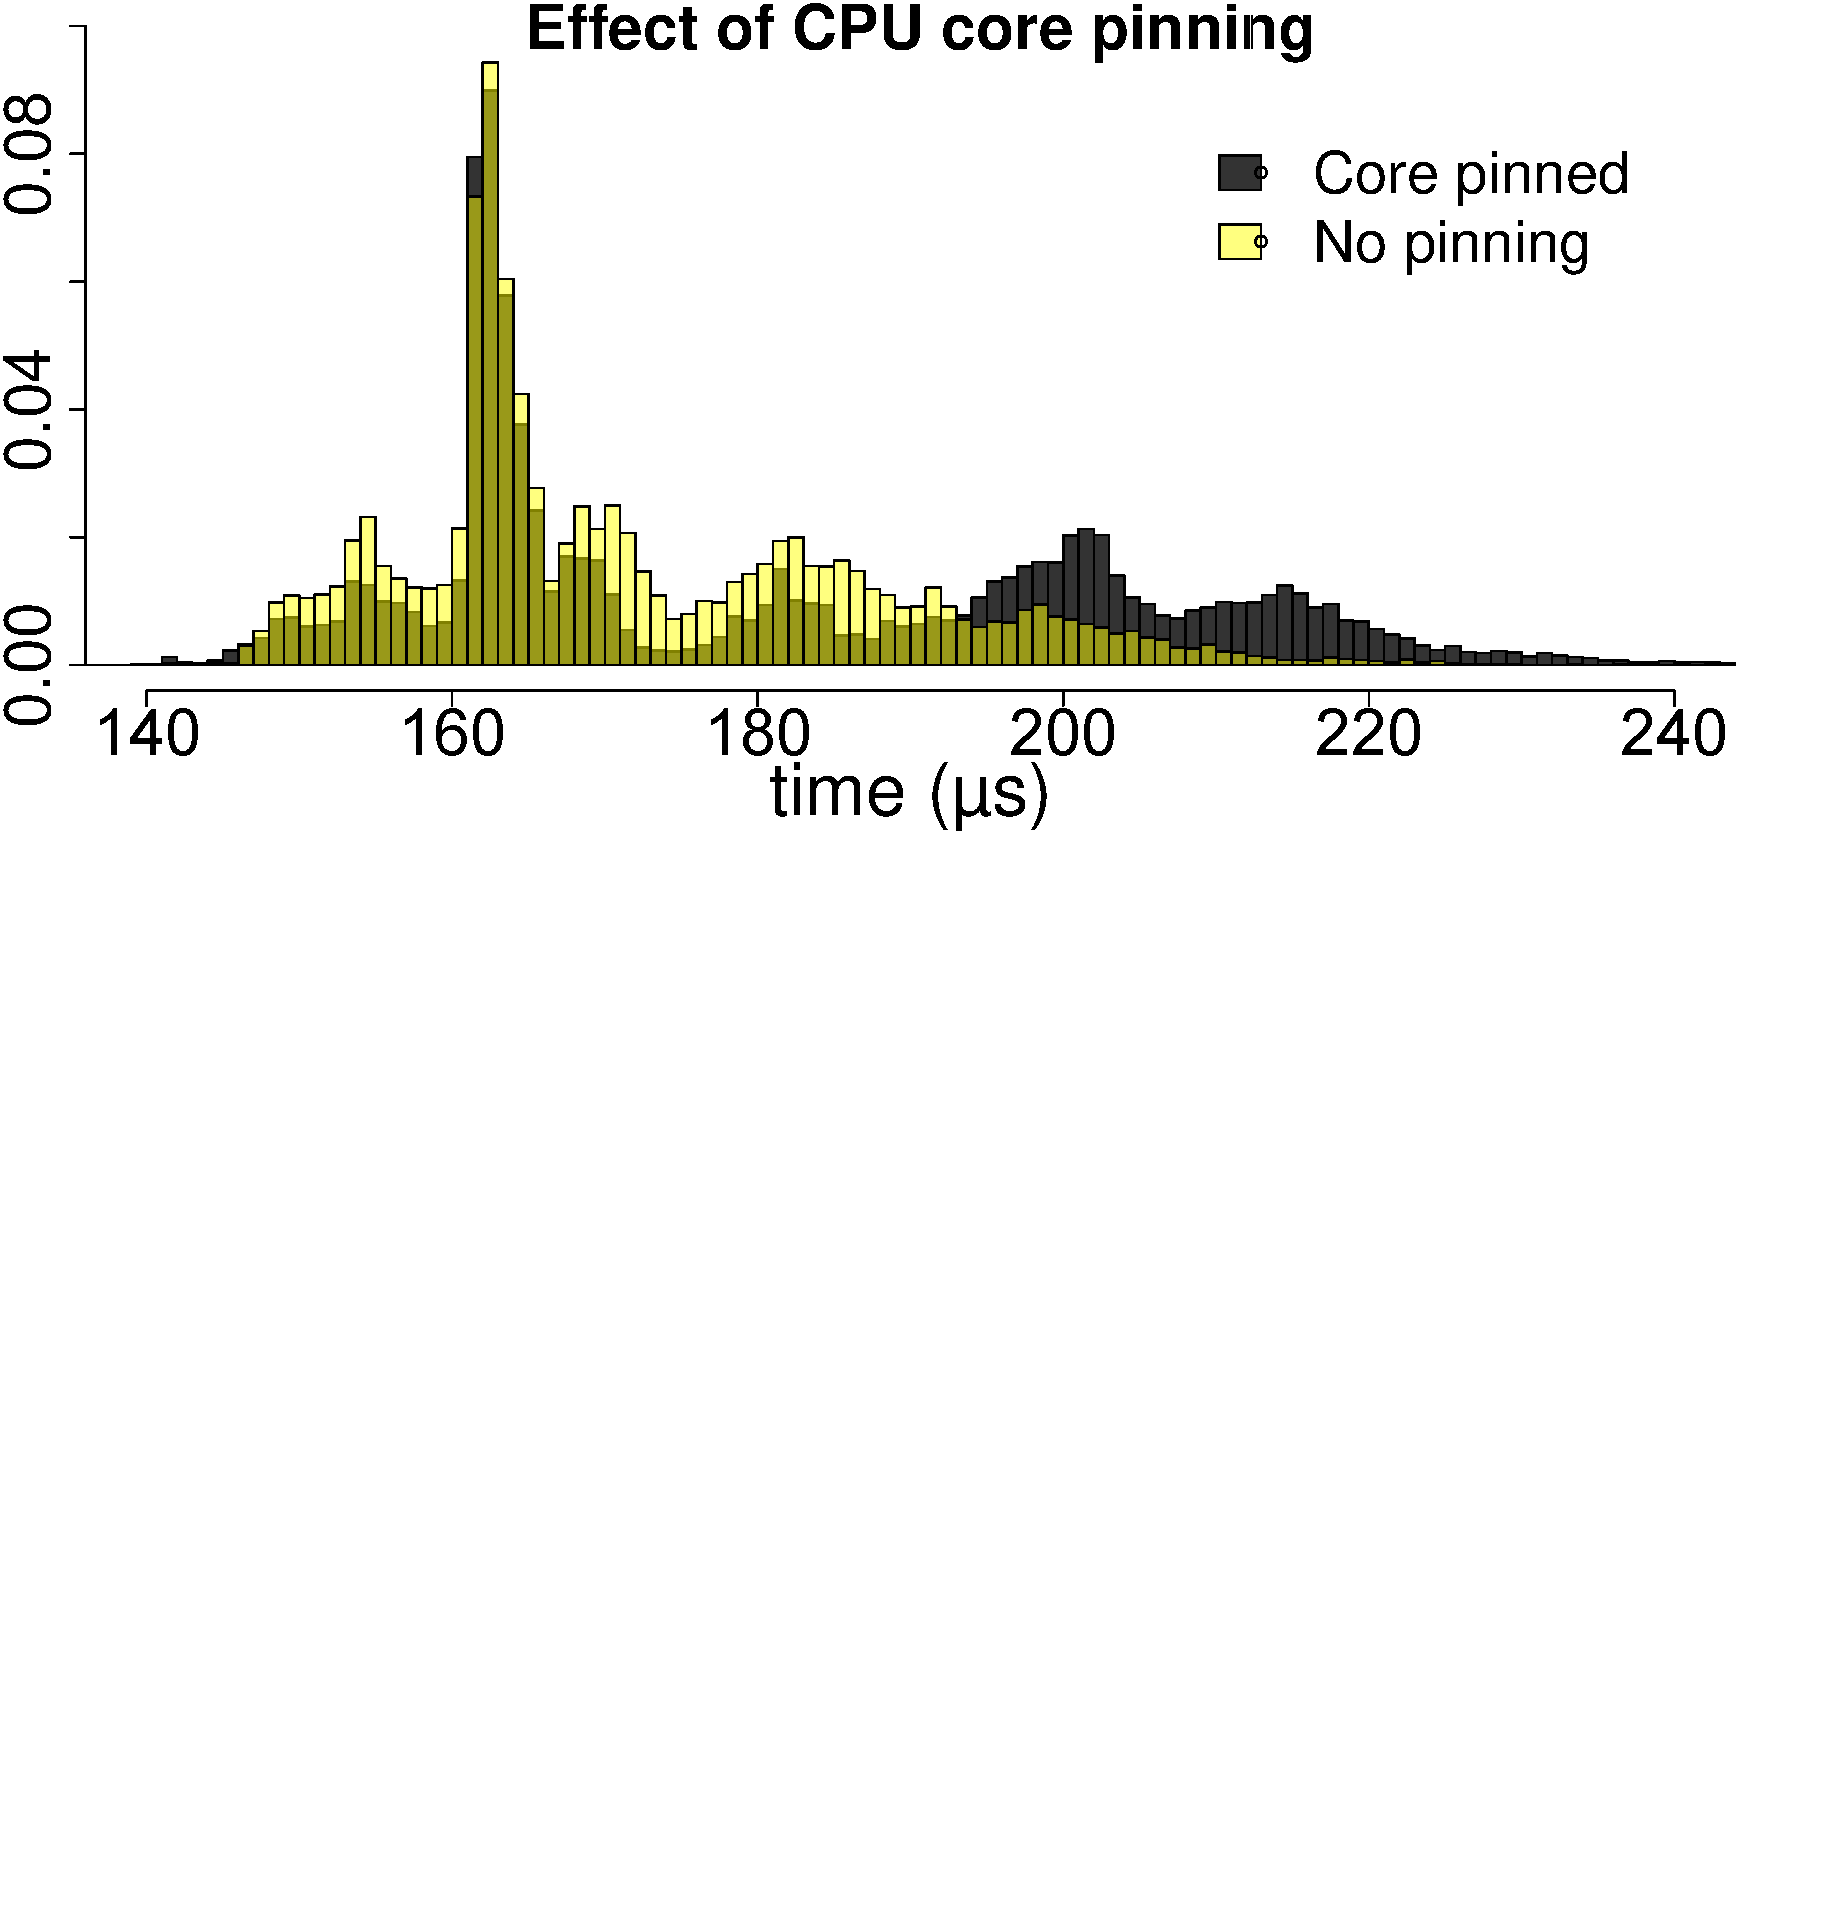
\includegraphics[trim={0 18cm 1.8cm 0}, clip, width=0.75\linewidth]{data/CPU_stress/plot_pin_1.pdf}
    \caption{\textbf{Effect of CPU core pinning on the enclave application.} Restricting the enclave application to a specific core has a very minor effect on the observed latency.}
    \figsaver
    \label{graph:cpuPin}
\end{figure}

\blue{\myparagraph{Effects of core pinning.} We executes the \name enclave application pinning to specific CPU cores (using the command \texttt{taskset [COREMASK] [EXECUTABLE]}). Core pinning forces the operating system to use a specific set of CPU core(s) to execute a program. CPU pinning may significantly bring down execution time due to the elimination of core switching and ability to reuse L1 and L2 cache. Figure~\ref{graph:cpuPin} illustrates the effect of CPU core pinning vs. no pinning. We experience negligible effect by core pinning. Hence we conclude that the attacker won't gain any advantage by CPU core pinning.}


%\begin{figure}[t]
%  \centering
%    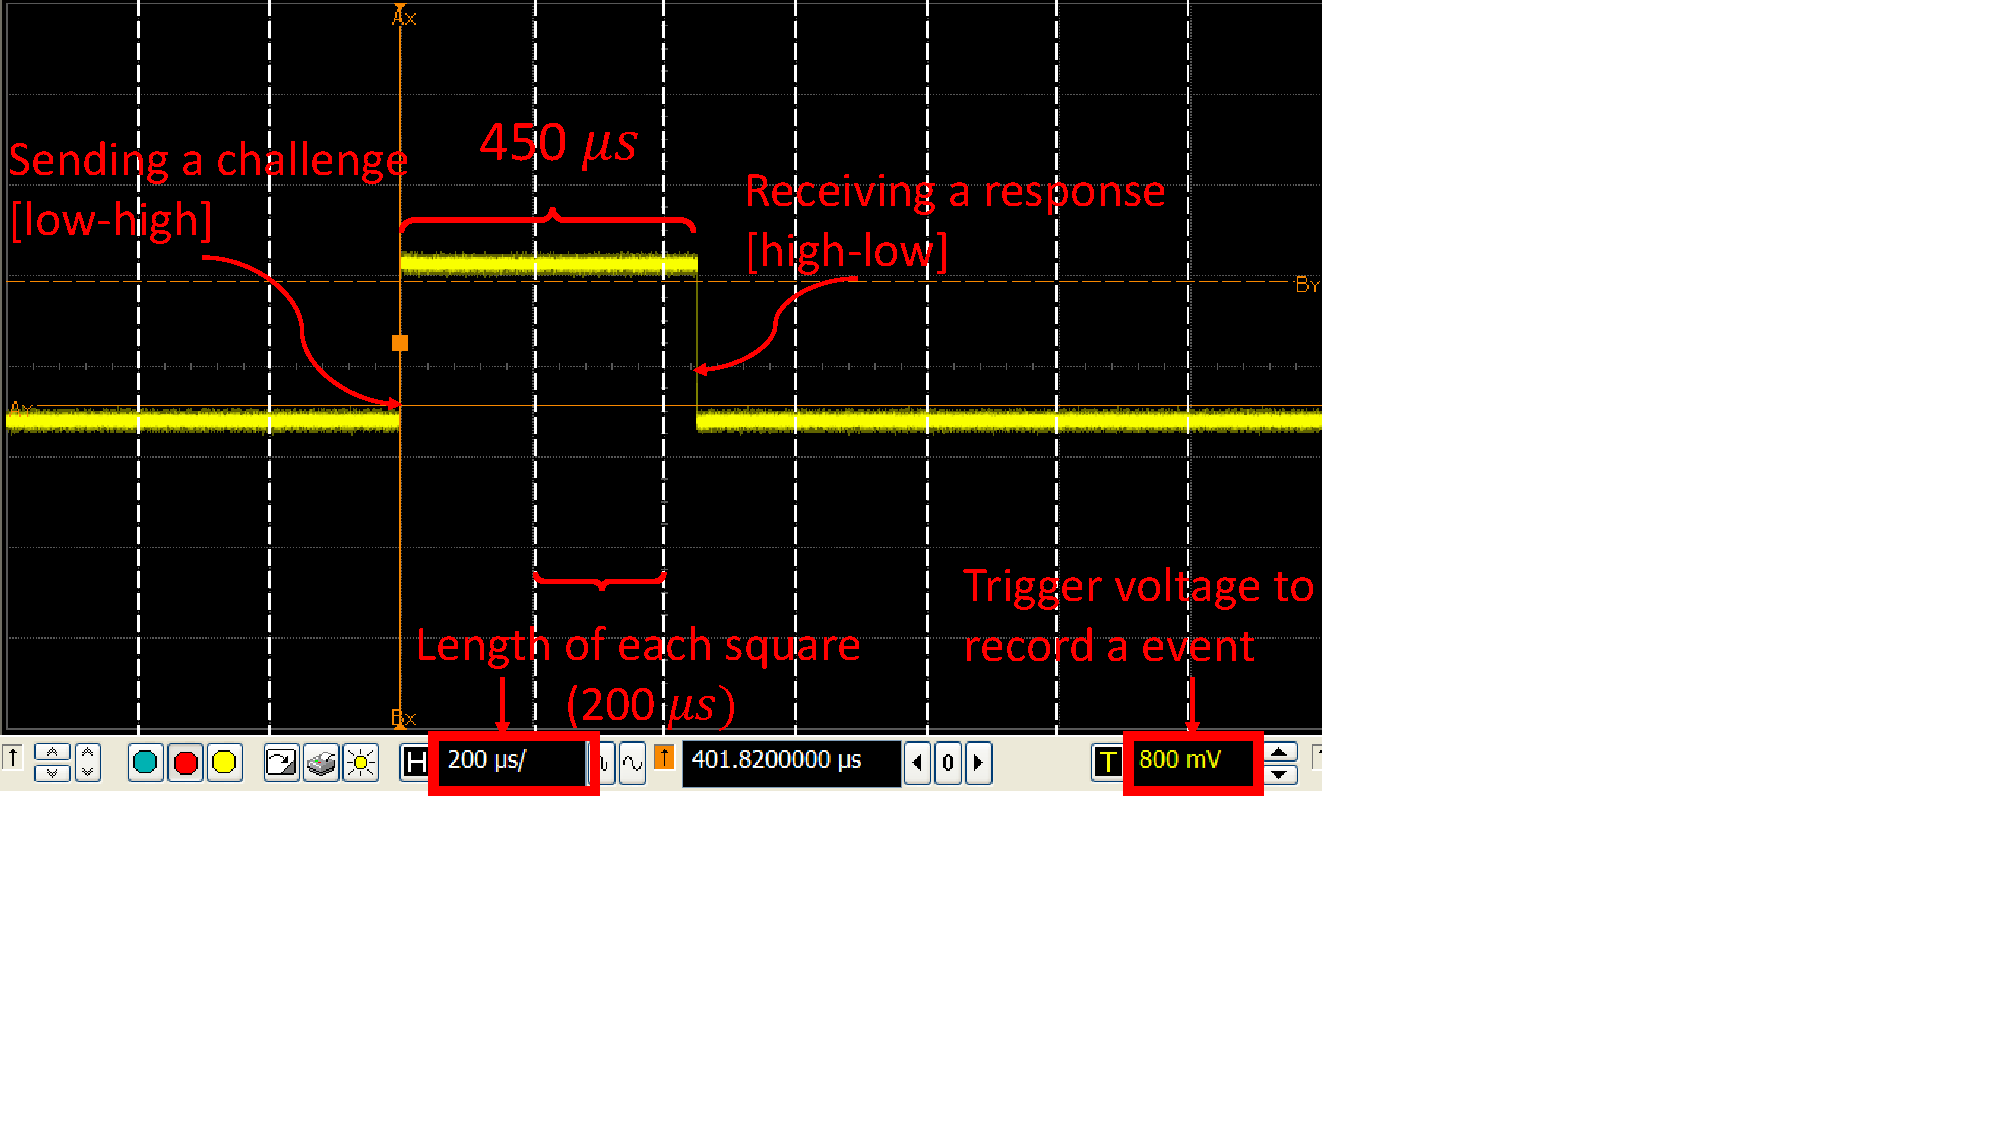
\includegraphics[trim={0 5.2cm 11cm 0}, clip, width=0.7\linewidth]{Osci.pdf}
%    \caption{\textbf{Latency measurement on oscilloscope.} We use a high precision oscilloscope to measure the latency of \name. The figure annotates the sending and the receiving of the challenge response messages that is activated by the GPIOs on the Arduino board.}
%    \label{fig:osci}
%\end{figure}

\iffalse
\begin{figure*}[t]
  \centering
    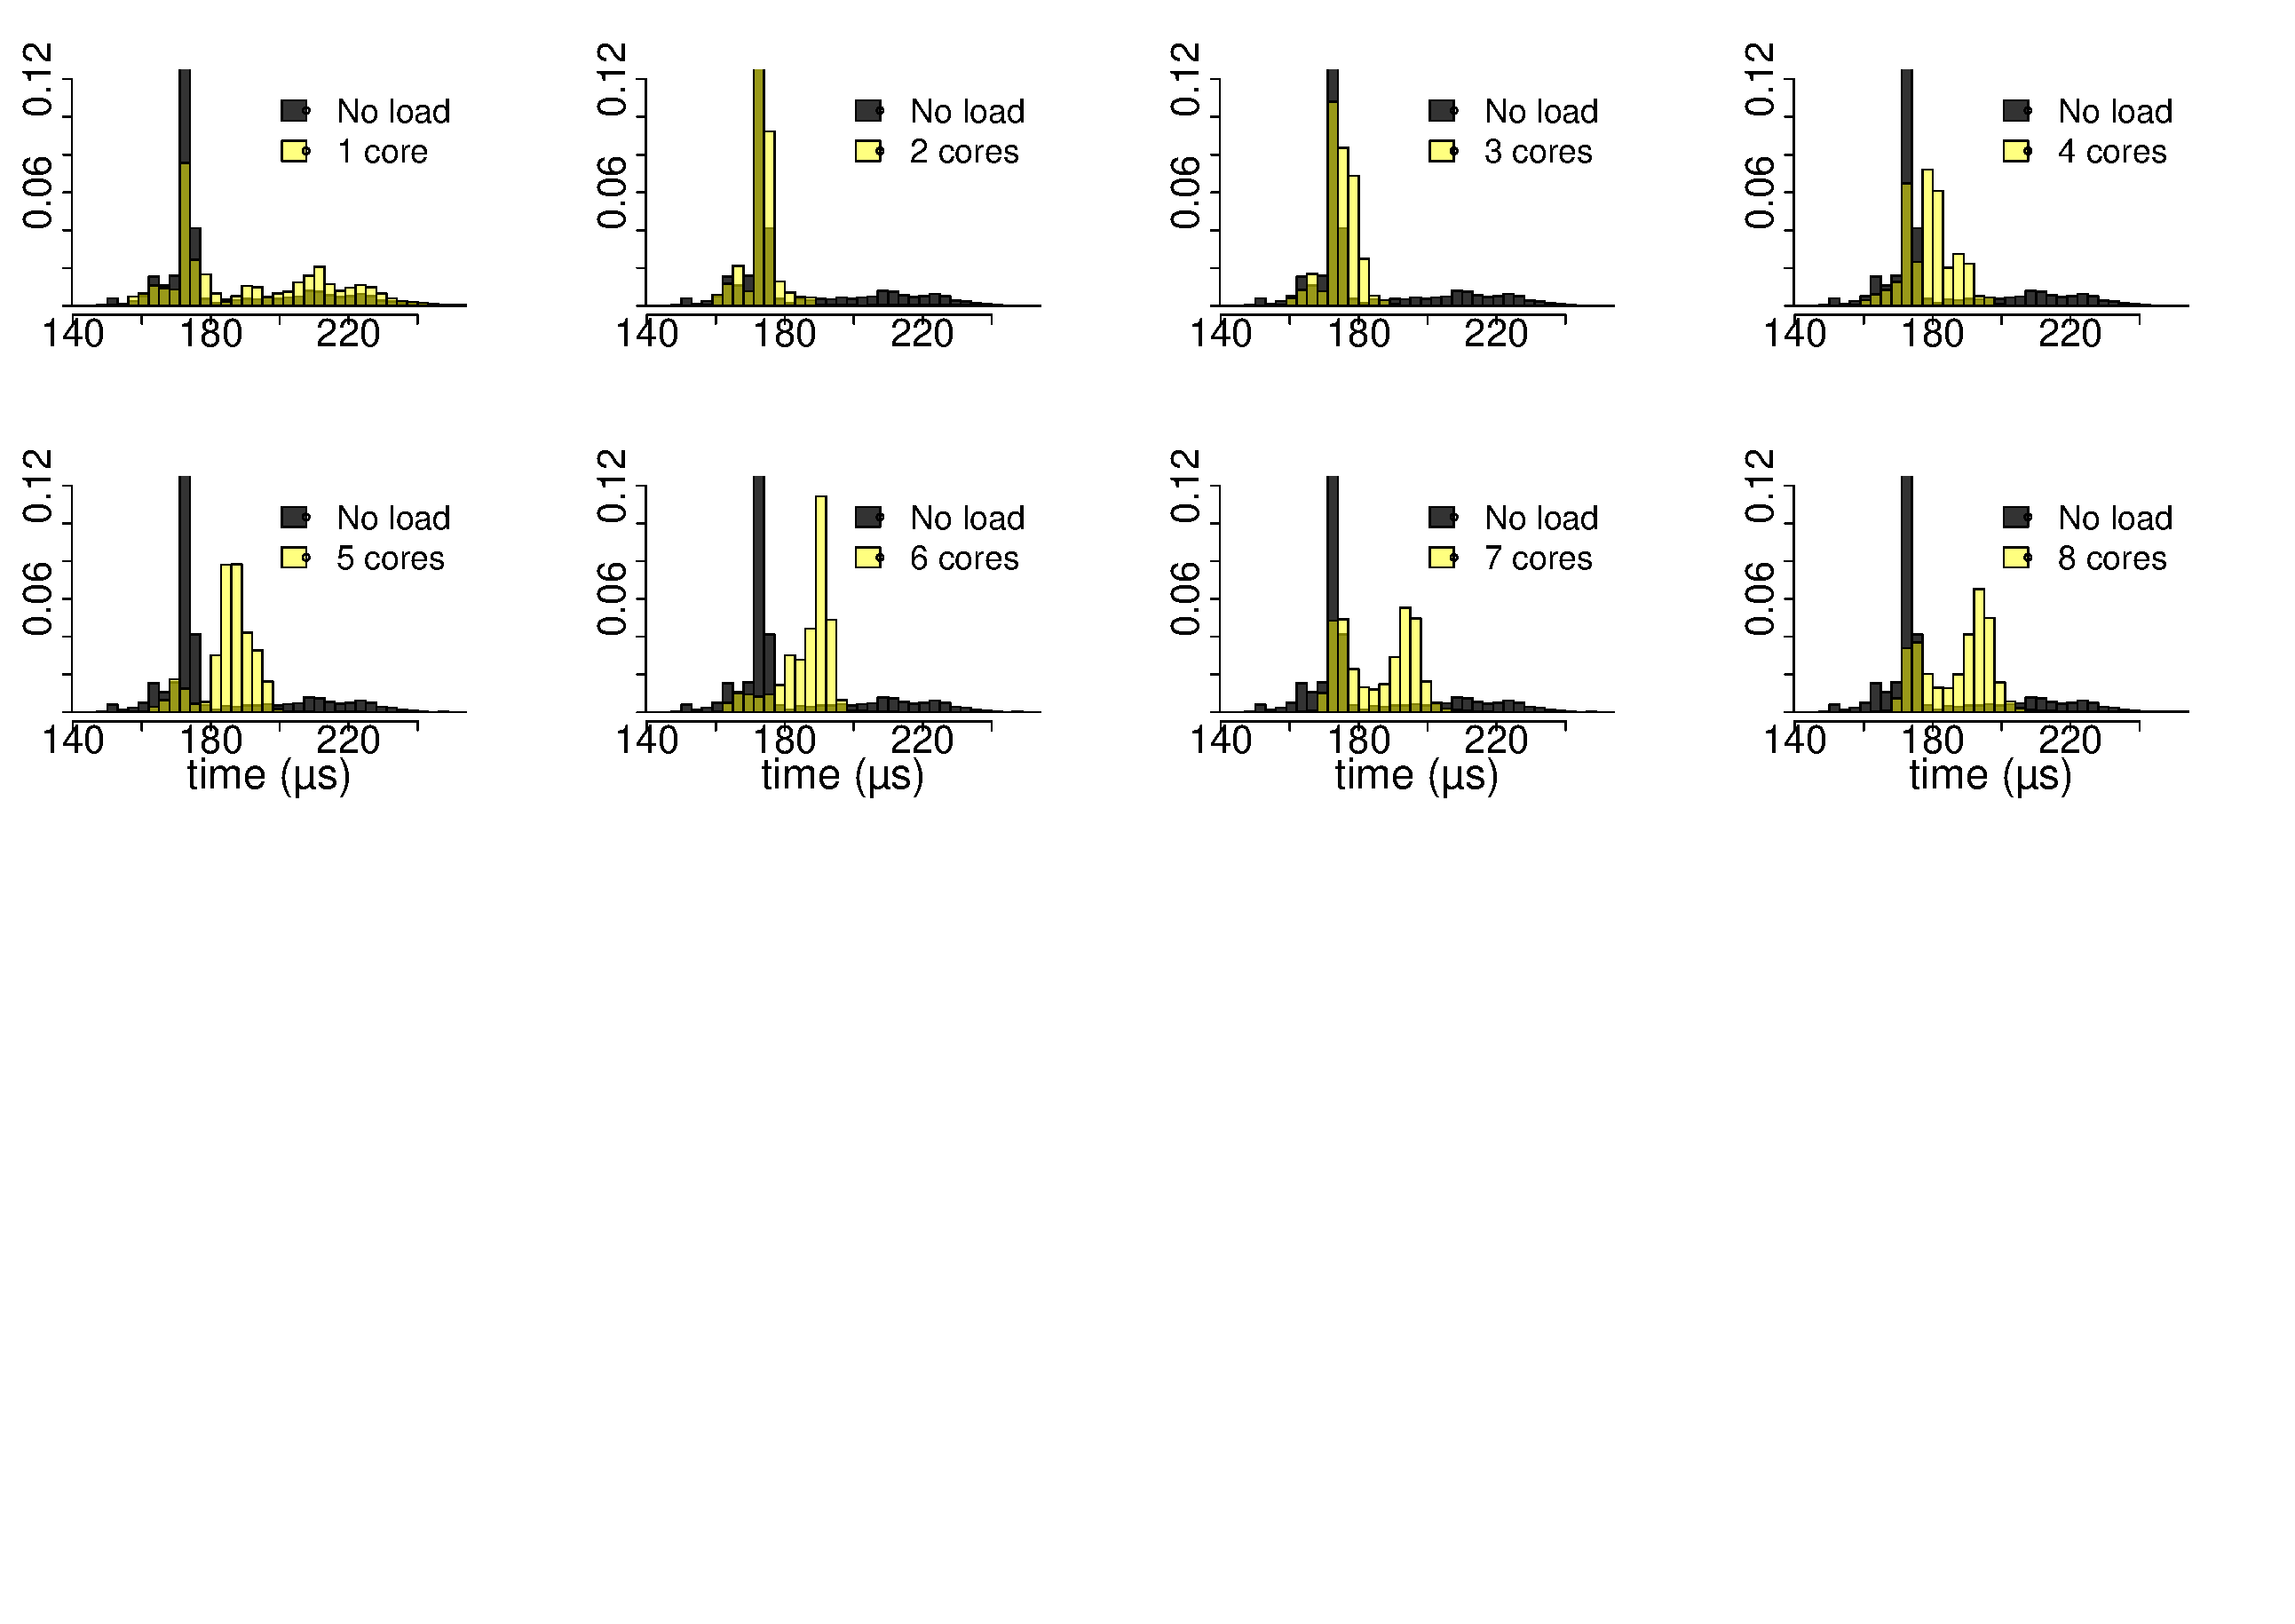
\includegraphics[trim={0 16cm 0 0}, clip, width=0.5\linewidth]{data/CPU_stress/allCore_1.pdf}
    \caption{\textbf{Effect on latency experienced by the \device with different number of stressed CPU cores.} We evaluated latencies while running CPU intensive benchmark on different number of cores. Note that with higher number of busy cores, the means of the  distributions start to shift towards right but stayed within \connect $= 186\mu s$. We used \texttt{stress-ng} Linux stress-testing application.}
    \label{graph:cpuLoad}
\end{figure*}
\fi

\begin{figure}[t]
  \centering
    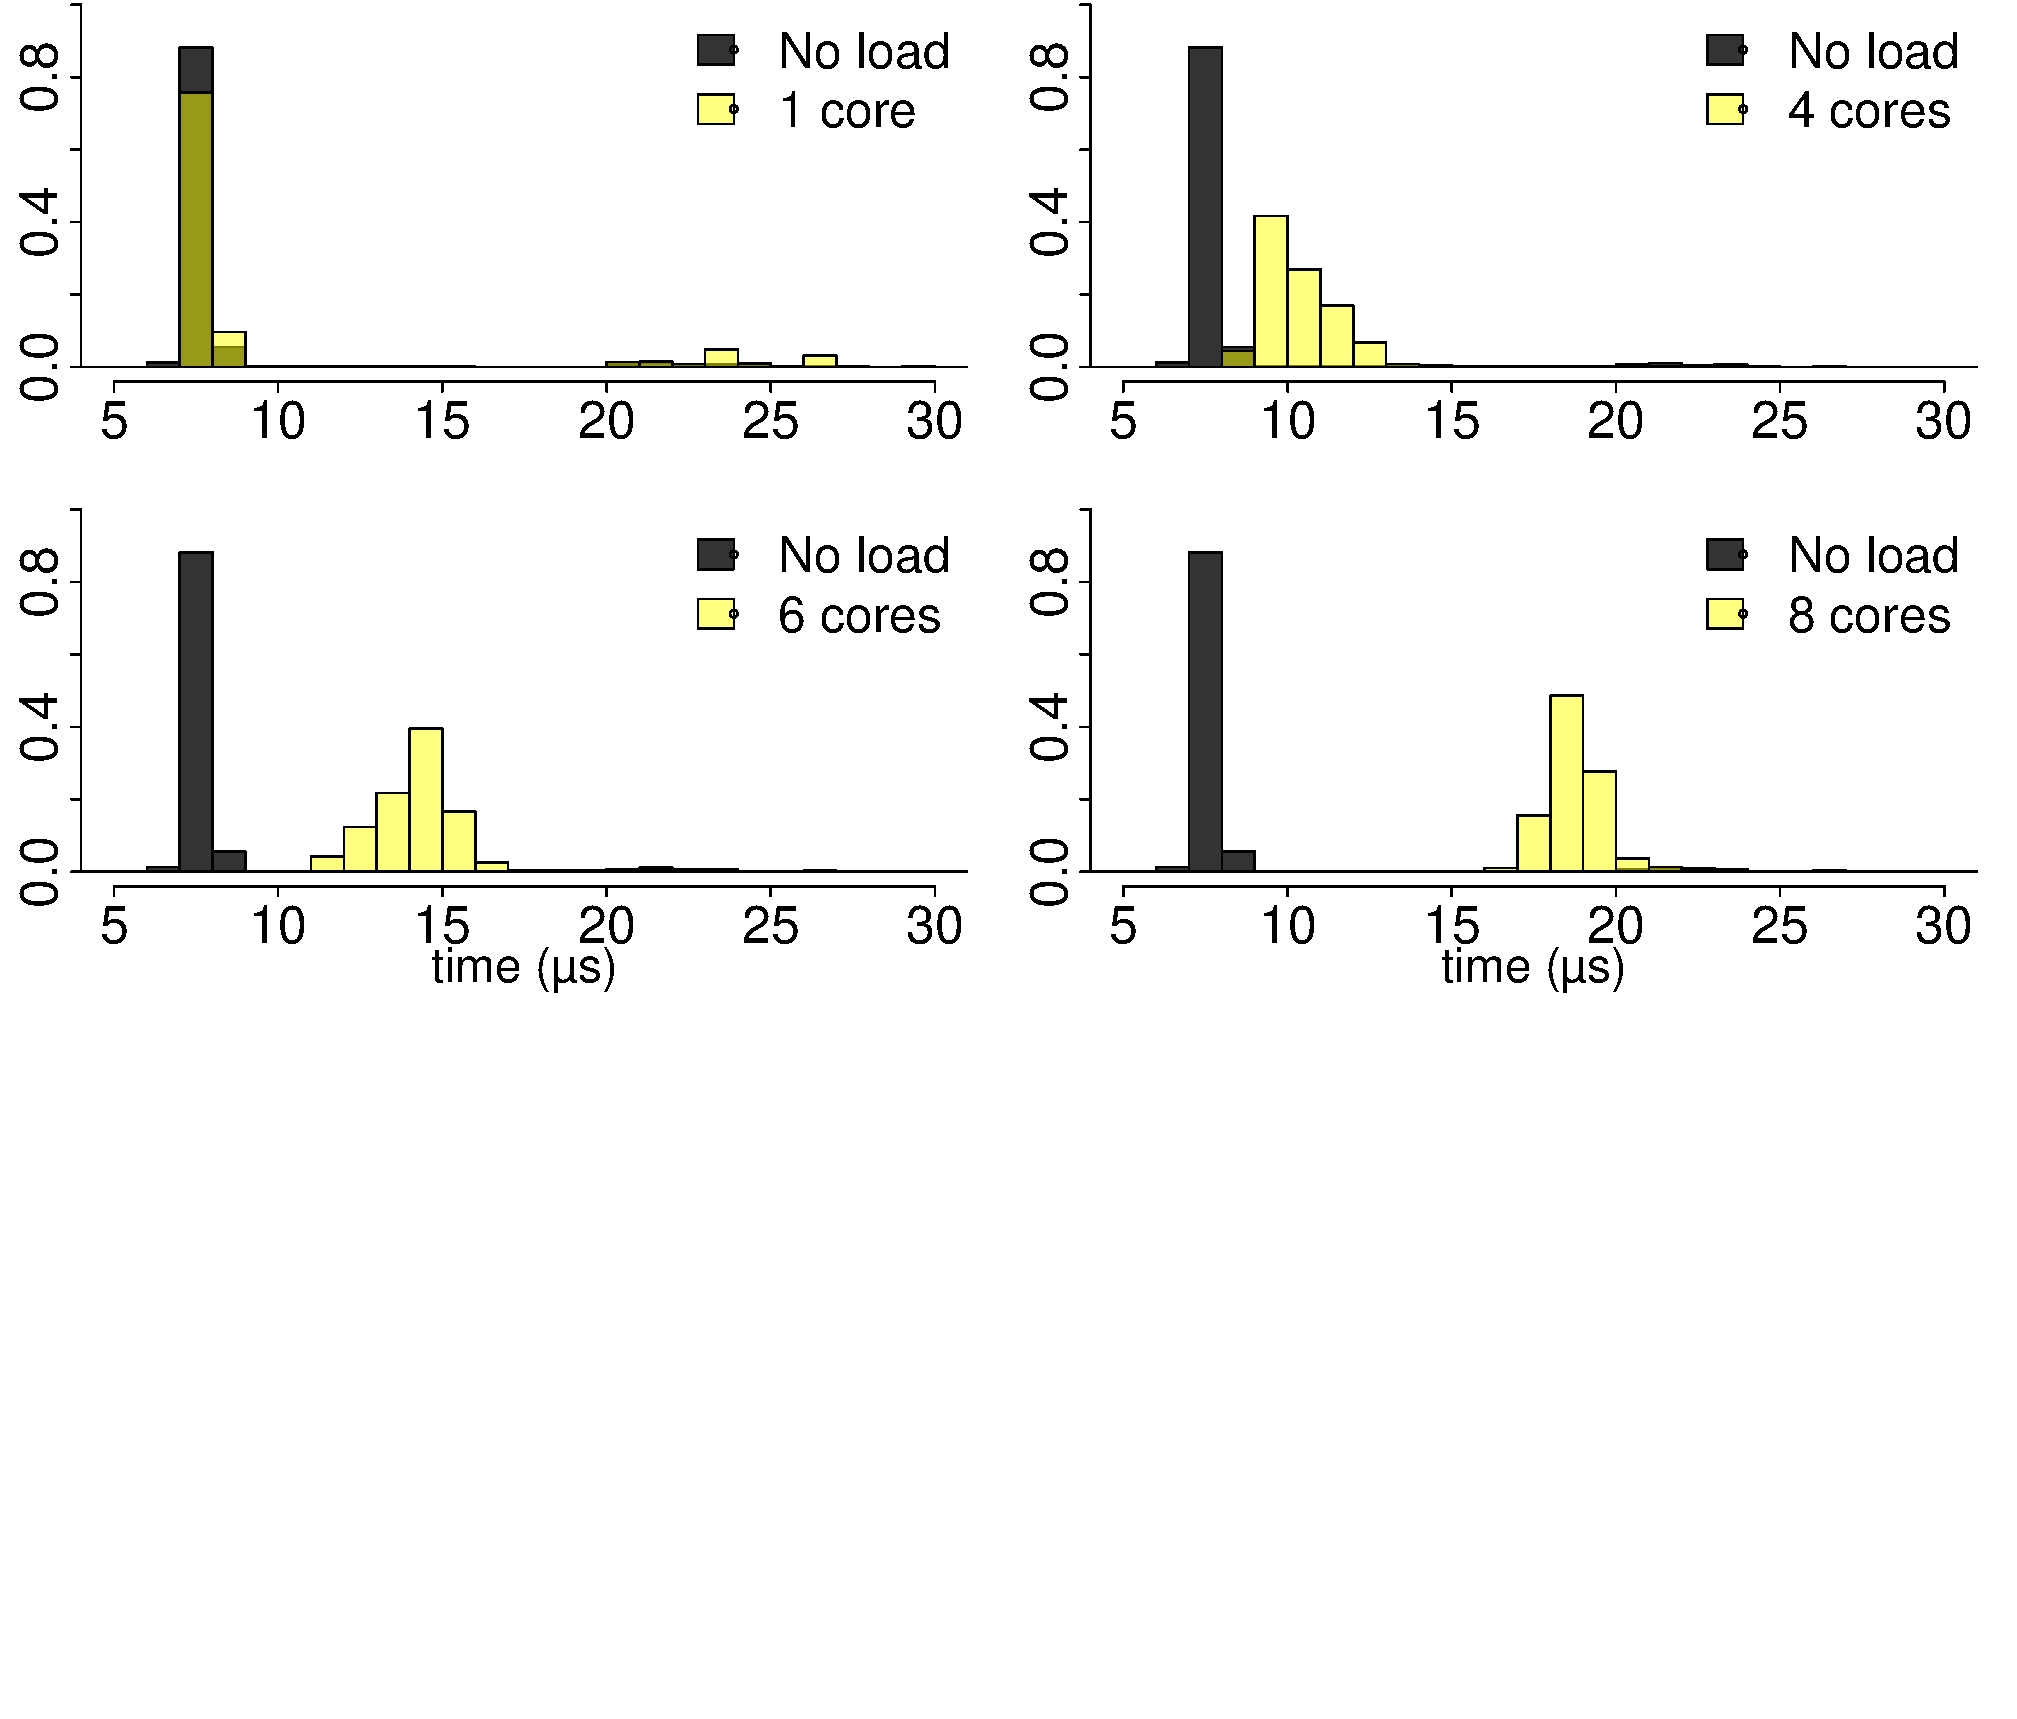
\includegraphics[trim={0 12cm 0 0}, clip, width=\linewidth]{data/CPU_stress/allCore_SGX_1.pdf}
    \caption{\textbf{Effect on enclave execution time with different number of stressed CPU cores.} Increase system load has a minor effect on observed enclave execution time.}
    \figsaver
    \label{graph:cpuLoad_SGX}
\end{figure}

\myparagraph{Effects of CPU load.} Figure~~\ref{graph:cpuLoad_SGX} shows the enclave execution times with varying degree of CPU stress testing. We used \texttt{stress-ng} to stress different number of CPU cores. We experienced a minor slowdown with the increasing number of busy CPU cores. But the slowdown is insignificant. For example, as shown in the Figure~\ref{graph:cpuLoad_SGX}, we experienced a shift of $12\mu s$ when all the 8 CPU cores are busy executing the benchmark software. Also, note that the load introduced by the benchmark is a sustained load on all the CPU cores which is much more demanding for the CPUs compared to the CPU loads introduced by real-life applications. In that scenarios, the deviation would be even lesser. We conclude that proximity verification for SGX enclaves is reliable even under high system load. In rare cases of extreme system load, proximity verification might fail, but this is an availability concern, not a security threat.


%\begin{figure}[t]
%  \centering
%    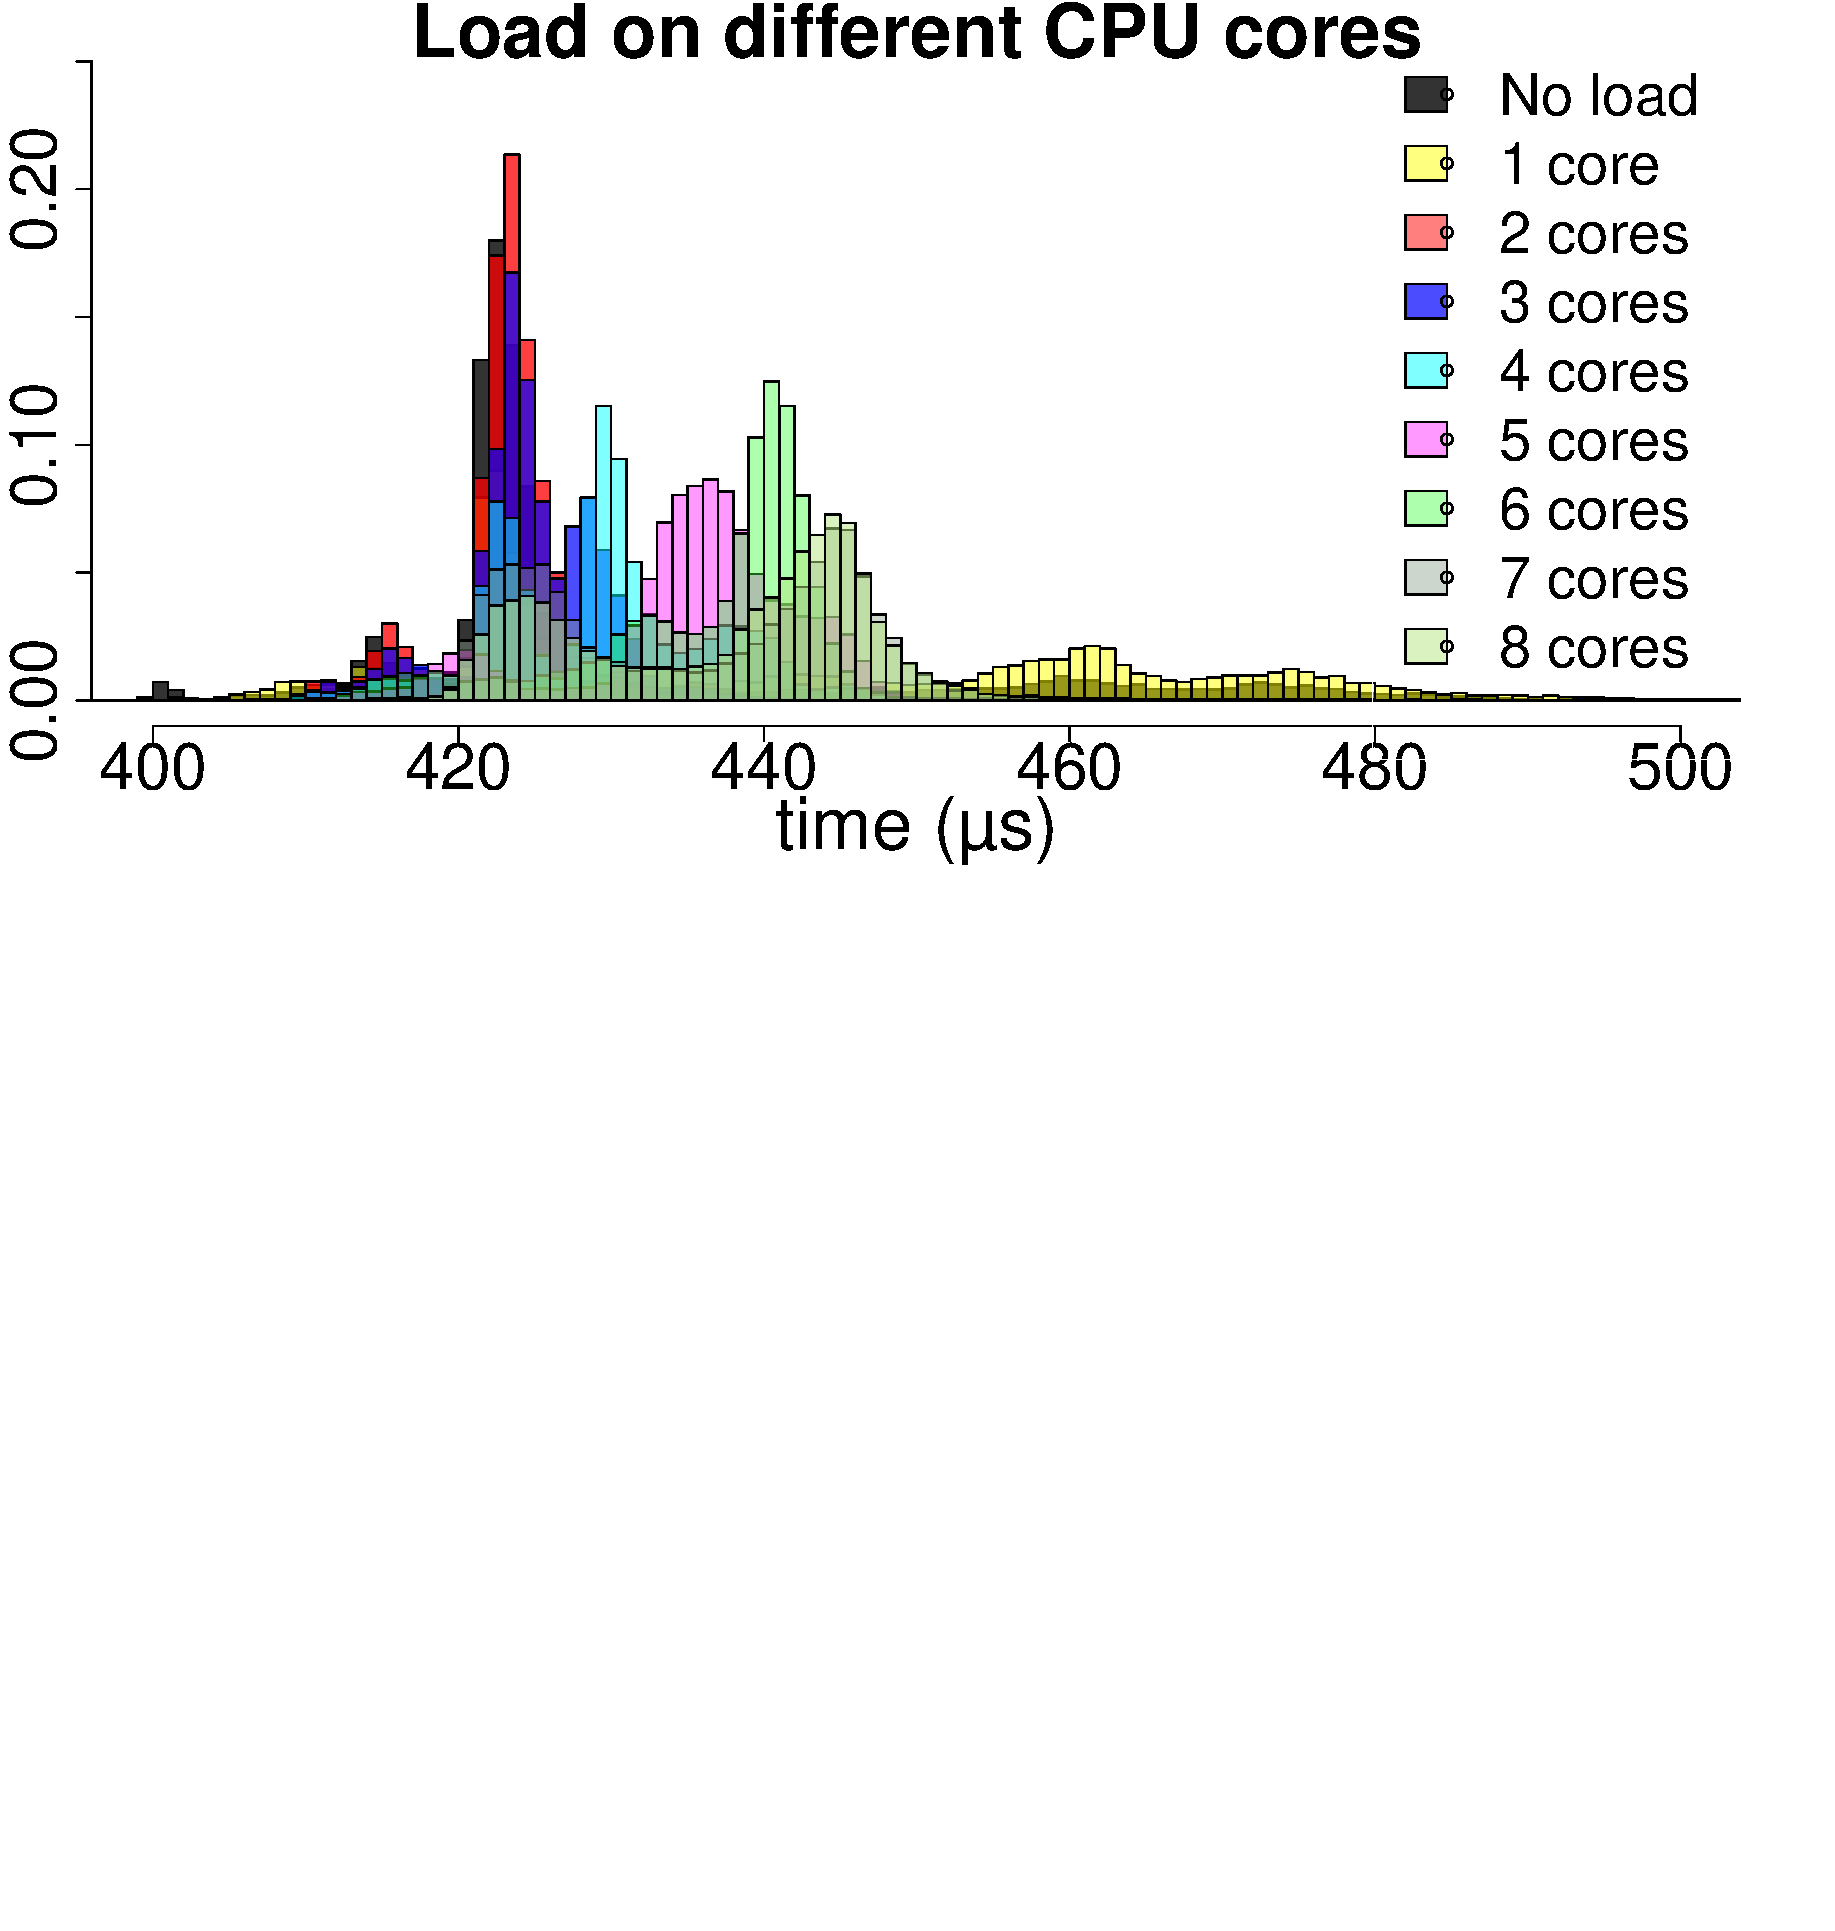
\includegraphics[trim={0 18cm 2cm 0}, clip, width=0.8\linewidth]{data/CPU_stress/plot.pdf}
%    \caption{\textbf{Effect of CPU stress on different number of cores.} We evaluated latencies while running CPU intensive benchmark on different number of cores.}
%    %\vspace{-20pt}
%    \label{graph:cpuLoad}
%\end{figure}







